\documentclass{article}

%%%%%%%%%%%%%%%%%%%%%%%%%%%%%%%%%%%%%%%%%%%%%%%%%%%%%%%%%%%%%%%%%%%%%%%%%%%%%%%%
%% package setup
%%%%%%%%%%%%%%%%%%%%%%%%%%%%%%%%%%%%%%%%%%%%%%%%%%%%%%%%%%%%%%%%%%%%%%%%%%%%%%%%


\usepackage[shortlabels]{enumitem}
\usepackage{amsfonts,amsmath, soul, matlab-prettifier, bm, amsthm,enumitem,amssymb,multirow,float,mathtools,bbm,array,varwidth,hyperref,bm}
\usepackage[all]{xy}
\usepackage[margin=0.9in]{geometry}
\usepackage{graphicx}
\usepackage{mathtools, caption, dsfont, tikz-cd}
\usepackage{wrapfig}

% tikzpicture

\usepackage{pgfplots}
\pgfplotsset{compat=1.15}
\usepackage{mathrsfs}
\usetikzlibrary{arrows}


\mathchardef\mhyphen="2D


\raggedbottom

%%%%%%%%%%%%%%%%%%%%%%%%%%%%%%%%%%%%%%%%%%%%%%%%%%%%%%%%%%%%%%%%%%%%%%%%%%%%%%%%
%% operators and symbols
%%%%%%%%%%%%%%%%%%%%%%%%%%%%%%%%%%%%%%%%%%%%%%%%%%%%%%%%%%%%%%%%%%%%%%%%%%%%%%%%

% operators
\newcommand{\Hom}{\mathrm{Hom}}
\newcommand{\Ext}{\mathrm{Ext}}
\newcommand{\Ker}{\mathrm{Ker}}
\newcommand{\Pic}{\mathrm{Pic}}
\newcommand{\comp}{\mathrm{comp}}
\newcommand{\Proj}{\mathrm{Proj}}
\newcommand{\rk}{\mathrm{rk}}
\newcommand{\Spec}{\mathrm{Spec}}
\newcommand{\Sym}{\mathrm{Sym}}
\newcommand{\Frob}{\mathrm{Frob}}
\newcommand{\Gal}{\mathrm{Gal}}
\newcommand{\GL}{\mathrm{GL}}
\newcommand{\SL}{\mathrm{SL}}
\newcommand{\Ind}{\mathrm{Ind}}
\newcommand{\Rep}{\mathrm{Rep}}
\newcommand{\Aut}{\mathrm{Aut}}
\newcommand{\Res}{\mathrm{Res}}
\newcommand{\Smo}{\mathrm{Smo}}
\newcommand{\Span}{\mathrm{Span}}
\newcommand{\Frac}{\mathrm{Frac}}
\newcommand{\supp}{\mathrm{supp}}
\newcommand{\End}{\mathrm{End}}
\newcommand{\St}{\mathrm{St}}
\newcommand{\Top}{\mathrm{Top}}
\newcommand{\Ab}{\mathrm{Ab}}
\newcommand{\Set}{\mathrm{Set}}
\newcommand{\ad}{\mathrm{ad}}
\newcommand{\hht}{\mathrm{ht}}

\newcommand{\PGL}{\mathrm{PGL}}
\newcommand{\PSL}{\mathrm{PSL}}
\newcommand{\Psh}{\mathrm{Psh}}
\newcommand{\Sh}{\mathrm{Sh}}
\newcommand{\Id}{\mathrm{Id}}
\newcommand{\aff}{\mathrm{aff}}


% greek 
\newcommand{\calpha}{\check{\alpha}}
\newcommand{\cPhi}{\check{\Phi}}
\newcommand{\cbeta}{\check{\beta}}
\newcommand{\valpha}{\alpha^\vee}
\newcommand{\vbeta}{\beta^\vee}
\newcommand{\vPhi}{\Phi^\vee}

% shortcuts
\newcommand{\slii}{\mathfrak{sl}_2}
\newcommand{\sliii}{\mathfrak{sl}_3}
\newcommand{\gl}{\mathfrak{gl}}
\newcommand{\eW}{\widetilde{W_a}}


% mathcal
\newcommand{\cO}{\mathcal{O}}
\newcommand{\cR}{\mathcal{R}}
\newcommand{\cH}{\mathcal{H}}

% mathbb
\newcommand{\CC}{\mathbb{C}}
\newcommand{\FF}{\mathbb{F}}
\newcommand{\NN}{\mathbb{N}}
\newcommand{\PP}{\mathbb{P}}
\newcommand{\QQ}{\mathbb{Q}}
\newcommand{\RR}{\mathbb{R}}
\newcommand{\ZZ}{\mathbb{Z}}
\newcommand{\GG}{\mathbb{G}}
\newcommand{\adele}{\mathbb{A}}
\newcommand{\pp}{\mathfrak{p}}
\newcommand{\nn}{\mathfrak{n}}
\newcommand{\mm}{\mathfrak{m}}

% mathfrak
\newcommand{\fg}{\mathfrak{g}}
\newcommand{\fh}{\mathfrak{h}}
\newcommand{\fm}{\mathfrak{m}}

% shortcuts
\newcommand{\CG}{C_c^{\infty}(G)}
\newcommand{\cInd}{c\mhyphen\mathrm{Ind}}

\newcommand{\norm}[1]{\left\lVert#1\right\rVert}
\newcommand{\hatv}[1]{\overset{\vee}{\mathstrut#1}}

\DeclareMathOperator{\Ima}{Im}

\linespread{1.5}

\theoremstyle{plain}
\newtheorem{theorem}{Theorem}[section]
\newtheorem{question}[theorem]{Question}
\newtheorem{proposition}[theorem]{Proposition}
\newtheorem{convention}[theorem]{Convention}
\newtheorem{lemma}[theorem]{Lemma}
\newtheorem{cor}[theorem]{Corollary}
\newtheorem{algo}[theorem]{Algorithm}
\theoremstyle{definition}
\newtheorem{definition}[theorem]{Definition}
\newtheorem{notn}[theorem]{Notation}
\newtheorem{remark}[theorem]{Remark}
\newtheorem{example}[theorem]{Example}
\newtheorem{examples}[theorem]{Examples}
\newtheorem{fact}[theorem]{Fact}
\newtheorem*{hypothesis}{Hypothesis}
\newtheorem*{exercise}{Exercise}


\title{Quadratic Relations in Hecke Algebras}
\author{Albert Lopez Bruch}

\begin{document}
	\maketitle
	\pagenumbering{arabic}
    %\section{Smooth representations and the Bernstein decomposition}

    Throughout this document, we let $F$ denote an arbitrary $p$-adic field with ring of integers $\mathcal{O}$, and residue field $k_F$ of characteristic $p>0$. Let $q=p^m$ be the cardinality of $k_F$ and let $\varpi$ be a uniformizer.

    Let $G$ denote a connected reductive group, defined and split over $\mathcal{O}$. The group $G(F)$ has a natural locally profinite topology coming from $F$. Fix an $F$-split
    maximal torus $T$ and a Borel subgroup $B$ containing $T$; assume $T$ and $B$ are defined over $\mathcal{O}$. Let $T_0=T(\mathcal{O})$ denote the maximal compact subgroup of $T(F)$. Let $\Phi\subset X^*(T)$ resp. $\Phi^\vee \subset X_*(T)$ denote the set of roots resp. coroots for $G$, $T$. Let $U$ resp. $\bar{U}$ denote the
    unipotent radical of $B$ resp. the Borel subgroup $\bar B \subset T$ opposite to $B$.

    %Let $\mathcal{B}(G,F)$ be the building of $G$ and let $\mathcal{A}(G,T,F)=X_*(T)\otimes\RR\subseteq \mathcal{B}(G,F)$ be the apartment corresponding to $T$, which comes equipped with a hyperplane structure arising from the affine roots. Let 
    %$$I=\langle T(\mathcal{\mathcal{O}}); \mathfrak{X}_\alpha(\mathcal{O}),\mathfrak{X}_{-\alpha}(\varpi\mathcal{O})\ |\ \alpha\in\Phi^+\rangle$$
    %be the Iwahori subgroup of $G$, and let $\textbf{a} \subset\mathcal{A}(G,T,F)$ be the unique alcove such that $G_{x,0}=I$ (first element in the Moy--Prasad filtration) for all $x\in\bf a$.

    Let $C$ be an algebraically closed field of characteristic $\ell\neq p$ and let $\cR_{C}(G)$ be the category smooth $C$-representations of $G$. That is, the objects of $\cR_{C}(G)$ are group homomorphisms $\pi: G\rightarrow GL(V)$ where $V$ is a $C$-vector space such that $\mathrm{Stab}_G(v)$ is an open subgroup of $G$ for all $v\in V$ (with respect to the locally profinite topology induced from $F$). If $V$ is finite dimensional, then the last condition is equivalent to $\ker\pi$ being open in $G(F)$. 

    If $C=\CC$, then the category $\cR_\CC(G)$ has a canonical decomposition. To state it, we consider the set of \textit{supercuspidal pairs} $(M,\sigma)$ where $M$ is an $F$-Levi subgroup of $G$ and $\sigma$ is a supercuspidal representation of $G$. 
    We say that two supercuspidal pairs $(M_1,\sigma_1)$ and $(M_2,\sigma_2)$ are \textit{inertially equivalent} if there exists some $g\in G(F)$ and \textit{unramified character} $\chi$ of $M_2$ such that $gM_1g^{-1}=M_2$ and $\prescript{g}{}{\sigma_1}\otimes\chi\cong \sigma_2$ as representations of $M_2$. We denote by $[M,\sigma]_G$ the conjugacy class of the pair $(M,\sigma)$, and we note that it is a union of $G$-conjugacy classes of supercuspidal pairs. Finally, let $\mathfrak{J}(G)=\{(M,\sigma)\text{ supercuspidal}\}/\sim$, where $\sim$ is inertial equivalence.

    If $(\pi,V)\in R_\CC(G)$ is irreducible, then there is some supercuspidal pair $(M,\sigma)$, unique up to $G$-conjugacy, such that $\pi$ is a subquotient of $i_P^G(\sigma)$, where $P=N\rtimes M$ is the unique parabolic subgroup with Levi factor $M$ and $i_P^G$ is the normalized parabolic induction. We call the $G$-conjugacy class $(M,\sigma)_G$ the supercuspidal support of $(\pi,V)$. For each $[M,\sigma]_G\in\mathfrak{J}(G)$, we define $\cR_{[M,\sigma]}(G)$ to be the full subcategory of $\cR_\CC(G)$ whose objects are smooth representations $(\pi,V)$ such that for all irreducible subquotients $\pi'$ of $\pi$, the supercuspidal support of $\pi'$ lies in $[M,\sigma]_G$.

    \begin{theorem}[Bernstein Decomposition]
        The category $\cR_\CC(G)$ has a block decomposition into full subcategories
        $$\cR_\CC(G)=\prod_{[M,\sigma]\in\mathfrak{J}(G)}\cR_{[M,\sigma]}(G).$$
    \end{theorem}
    
    \begin{remark}
        In any abstract category of representations $\cR(G)$ of a group $G$ with certain properties (smoothness, for instance) such that the category is closed under direct sums and extensions, one can always decompose $\cR(G)$ into maximal blocks as follows:

        Firstly, we consider an equivalence relation on irreducible representations of $\cR(G)$ generated by the rule that two irreducible representations $(\pi_1,V_1)$ and $(\pi_2,V_2)$ are related if there is some representation $(\sigma,W)\in\cR(G)$ and non-split short exact sequence
        $$0\longrightarrow (\pi_1,V_1)\longrightarrow(\sigma,W)\longrightarrow(\pi_2,V_2)\longrightarrow 0.$$
        For any irreducible $(\pi,V)$ we let $\cR_{[\pi,V]}(G)$ to be the full subcategory of representations such that all simple Jordan-Holder factors are equivalent to $(\pi,V)$ under $\sim$.
        \begin{theorem}
            The category $\cR(G)$ admits a block decomposition into full subcategories 
            $$\cR(G)=\prod_{[\pi,V]}\cR_{[\pi,V]}(G)$$
        \end{theorem}
        The Theorem is direct consequence of the following result.
        \begin{proposition}
            Let $(\sigma,W)\in\cR_{[\pi,V]}(G)$ and $(\sigma',W')\in\cR_{[\pi',V']}(G)$. If $(\pi,V)\not\sim(\pi',V')$, then there are no non-trivial extensions of $(\sigma',W')$ by $(\sigma,W)$. 
        \end{proposition}
        \begin{proof}
            To be written, check the notebook.
        \end{proof}
    \end{remark}

    %\newpage
    %\section{Bernstein blocks, types and Hecke algebras}
    The Bernstein decomposition states that to understand $\cR(G)$, it is enough to understand $\cR_{[M,\sigma]}(G)$ for each $[M,\sigma]\in\mathfrak{J}(G)$. One can then understand each block using the theory of \textit{types}. 
    \begin{definition}
        Let $[M,\sigma]\in\mathfrak{J}(G)$. A pair $(K,\rho)$ consisting of a compact open subgroup $K$ of $G(F)$ and an irreducible smooth representation $\rho$ of $K$ is an $[M,\sigma]$-type if for any $(\pi,V)\in \cR_\CC(G)$, the following are equivalent:
        \begin{enumerate}
            \item $(\pi,V)\in\cR_{[M,\sigma]}(G).$
            \item $\Hom_K(\rho,\pi|_K)\neq\{0\}$; that is, $\rho\subseteq \pi|_K$.
        \end{enumerate}
    \end{definition}

    \begin{theorem}
        If $(K,\rho)$ is an $[M,\sigma]$-type, then the functor 
        \begin{align*}
            \cR_{[M,\sigma]}(G)&\longrightarrow \End_{G(F)}(\cInd_K^{G(F)}\rho)^{op}-\textrm{mod}\\
            (\pi,V)&\longmapsto\Hom_K(\rho,\pi|_K)
        \end{align*}
        is an equivalence of categories between the block $\cR_{[M,\sigma]}(G)$ and the category of right $\End_{G(F)}(\cInd_K^{G(F)}\rho)$-modules. 
    \end{theorem}
    We note that by Frobenius reciprocity, $$\Hom_K(\rho,\pi|_K)\cong\Hom_{G(F)}(\cInd_K^{G(F)}\rho,\pi),$$ so the former is naturally a right $\End_{G(F)}(\cInd_K^{G(F)}\rho)$-module, since it acts on the latter by precomposition.

    The idea of the proof is to show that if $(K,\rho)$ is a $[M,\sigma]$-type, then $\cInd_K^{G(F)}\rho$ is a projective generator of 
    $\cR_{[M,\sigma]}(G)$, and that the block is equivalent to the full subcategory $\cR_\rho(G)$ whose objects are representations $(\pi,V)$ satisfying $V=V[\rho]$, where $V[\rho]$ is the $G$-submodule of $V$ generated by its $\rho$-isotypical component $V^\rho$. The result then follows by the Morita equivalence. 

    In addition, the Hecke algebra $\End_{G(F)}(\cInd_K^{G(F)}\rho)$ can be described alternatively as a space of functions on $G$ valued on $\End_\CC(W)$, where $W$ is the vector space upon which $\rho$ acts.

    Let $\cH(G,K,\rho)$ denote the space of compactly supported functions $$\varphi:G\longrightarrow\End_\CC(W)$$
    satisfying
    $$\varphi(k_1 g k_2)=\rho(k_1)\circ\varphi(g)\circ\rho(k_2)$$
    for all $k_1,k_2\in K$ and $g\in G(F)$, equipped with a binary operation called \textit{convolution} as follows. If $\varphi_1,\varphi_2\in\cH(G,K,\rho)$, we define the function $\varphi_1*\varphi_2\in\cH(G,K,\rho)$ as
    $$\varphi_1*\varphi_2(g)=\sum_{h\in G(F)/K}\varphi_1(h)\varphi_2(h^{-1}g)=\int_{G(F)}\varphi_1(h)\varphi_2(h^{-1}g)dh,$$
    for $g\in G(F)$, where $dh$ denotes a Haar measure on $G(F)$ chosen to have measure $1$ on $K$. This operation gives $\cH(G,K,\rho)$ the structure of an associative $\CC$-algebra, whose identity element is the function $e:G\to\End_\CC(W)$ supported on $K$ such that $e(k)=\rho(k)$ for all $k\in K$.

    \begin{proposition}
        There are mutually inverse $\CC$-algebra homomorphisms
        \begin{equation}
            \Phi\longmapsto \varphi_\Phi\ :\ \End_{G(F)}(\cInd_K^{G(F)}\rho)\longrightarrow\cH(G,K,\rho)\ :\ \varphi \longmapsto \Phi_\varphi
        \end{equation}
        where
        \begin{align*}
            &\varphi_\Phi(g)(w)=\Phi(e_w)(g)\quad & (g\in G(F), w\in W)\\
            &\Phi_\varphi(f)(g)=\int_{G(F)}\varphi(h)(f(h^{-1}g))dh \quad &(f\in\cInd_K^{G(F)}\rho, g\in G(F)).
        \end{align*}
        Here, the Haar measure $dh$ is chosen so that it has measure $1$ on $K$ and $e_w\in\cInd_K^{G(F)}\rho$ is defined by
        \begin{align*}
            e_w(g)=
            \begin{cases}
                \rho(g)(w) &\text{ if } g\in K,\\
                0 &\text{ otherwise.}.
            \end{cases}
        \end{align*}        
    \end{proposition}
    \begin{proof}
        Some of the important steps:
        \begin{itemize}
            \item The maps are inverses of each other: This follows from 
            $$\Phi_\varphi(e_w)(g)=\int_{gK}\varphi(h)(e_w(h^{-1}g))dh=\int_K\varphi(gk)(e_w(k^{-1}))dk=\int_K\varphi(g)\circ\rho(k)(\rho(k)^{-1}w)=\varphi(g)(w)$$
            and 
            $$\int_{G(F)}\varphi_\Phi(h)(e_w(h^{-1}g))dh=\int_{K}\varphi_\Phi(gk)(e_w(k^{-1}))dk=\int_{K}\varphi_\Phi(g)\circ\rho(k)(\rho(k)^{-1}w)dk=\varphi_\Phi(g)(w)=\Phi(e_w)(g).$$
        \end{itemize}
    \end{proof}

    %\newpage
    %\section{Depth-zero Hecke algebras for principal series blocks}
    Let $\cR_{[M,\sigma]}(G)$ be a Bernstein block. If $M$ is the maximal torus $T$ (or a conjugate of $T$), then $\sigma=\tilde\chi$ is just a character and the $\cR_{[T,\tilde\chi]}(G)$ is called a principal series block. These are the ones we aim to understand.

    We remark that the block is completely determined the values of $\tilde\chi$ on $T(\cO)$, which has a natural filtration of open compact subgroups
    $$T(\cO)\supset T(1+\varpi\cO)\supset T(1+\varpi^2\cO)\supset T(1+\varpi^3\cO)\supset\cdots$$
    which forms a basis for the topology at the identity.
    This motivates the following definition:
    \begin{definition}
        The \textit{depth} of $\chi$ is the smallest integer $r$ such that $\chi$ is trivial on $T(1+\varpi^{r+1}\cO)$.
    \end{definition}
    In particular, if $\chi$ has depth-zero, then $\chi$ is trivial on $T(1+\varpi\cO)$ and therefore it factors through the quotient $T(\cO)\rightarrow T(k_F)$. We shall abuse notation and denote the resulting character $T(k_F)\rightarrow \CC^{\times}$ also as $\chi$. Fortunately, for such blocks, the construction of a type is completely explicit.

    Recall that the Iwahori subgroup $I$ of $G$ is defined as 
    $$I=\langle T(\mathcal{\mathcal{O}}); \mathfrak{X}_\alpha(\mathcal{O}),\mathfrak{X}_{-\alpha}(\varpi\mathcal{O})\ |\ \alpha\in\Phi^+\rangle$$
    with its pro-$p$ unipotent radical
    $$I^+=\langle T(1+\varpi\mathcal{\mathcal{O}}); \mathfrak{X}_\alpha(\mathcal{O}),\mathfrak{X}_{-\alpha}(\varpi\mathcal{O})\ |\ \alpha\in\Phi^+\rangle.$$

    We remark that in using the root subgroups of $G$, we have implicitly chosen a Chevalley basis of $\mathfrak{g}$, the Lie algebra of $G$.

    %Let $\mathcal{B}(G,F)$ be the building of $G$ and let $\mathcal{A}(G,T,F)=X_*(T)\otimes\RR\subseteq \mathcal{B}(G,F)$ be the apartment corresponding to $T$, which comes equipped with a hyperplane structure arising from the affine roots. Let 
    %$$I=\langle T(\mathcal{\mathcal{O}}); \mathfrak{X}_\alpha(\mathcal{O}),\mathfrak{X}_{-\alpha}(\varpi\mathcal{O})\ |\ \alpha\in\Phi^+\rangle$$
    %be the Iwahori subgroup of $G$, and let $\textbf{a} \subset\mathcal{A}(G,T,F)$ be the unique alcove such that $G_{x,0}=I$ (first element in the Moy--Prasad filtration) for all $x\in\bf a$.

    In particular, there is an isomorphism
    $$T(\cO)/T(\cO)\cap I^+\cong I/I^+$$
    and therefore $\chi$ determines a character $\rho_\chi$ of $I$ that is trivial on $I^+$. Explicitly, $I$ has an Iwahori decomposition $$I=(I\cap\bar U)\cdot T(\cO)\cdot(I\cap U),$$
    and $\rho_\chi$ extends $\chi$ in $T(\cO)$ and is trivial on $I\cap\bar U$ and $I\cap U$.

    \begin{theorem}
        Suppose that $\chi$ is a depth-zero character of $T(\cO)$. Then $(I,\rho_\chi)$ is a $[T,\tilde\chi]$-type, where $\tilde\chi$ is any extension of $\chi$ to $T(F)$.
    \end{theorem}

    This theorem motivates us to study the Hecke algebra $\cH(G,I,\rho_\chi)$, where $\rho_\chi$ is a character of $I$ arising from a depth-zero character of $T(\cO)$ as described above. 

    When $C=\CC$ has characteristic $0$, one can explicitly describe the structure of $\cH(G,I,\rho_{\chi})$ in terms of a few objects associated to $\chi$. To state the theorem, we first need some preliminaries. Firstly, we let $N:=N_G(T)$ be the normalizer of the torus, and we let $W=N(F)/T(F)$ and $\tilde{W}=N(F)/T(\cO)$ be the Weyl group and the extended Weyl group of $G$ respectively. The Weyl group is a coxeter group generated by a set of simple reflections $S=\{s_\alpha\ |\ \alpha\in\Pi\}$, where $\Pi\subset\Phi$ is any fixed integral basis. There is also a canonical isomorphism of abelian groups $X_*(T)=\Hom_F(\GG_m,T)\longrightarrow T(F)/T(\cO)$ given by $\lambda\mapsto\lambda(\varpi^{-1})$.
    
    There is a canonical surjective homomorphism $\tilde{W}\rightarrow W$ with kernel $X_*(T)$ and a non-canonical section. Therefore there is a non-canonical isomorphism $\tilde{W}=X_*(T)\rtimes W$. The extended Weyl group $\tilde{W}$ comes with an action on the apartment $\mathcal{A}=\mathcal{A}(G,T,F)=X_*(T)\otimes\RR$ that respects the hyperplane structure and therefore permutes the alcoves. The apartment is effectively a vector space over $\RR$ where the origin is the only point fixed by every $s_\alpha,\ \alpha\in\Phi$. The group $X_*(T)$ acts naturally by translations and $W$ is the group of transformations of $\tilde{W}$ fixing the origin. Inside the apartment, we distinguish the Weyl chamber and fundamental alcove of $\Phi$ which are, respectively,
    \begin{align*}
        \mathcal{C}&=\{v\in\mathcal{A}\ |\ 0<\langle\alpha,v\rangle,\forall\alpha\in\Phi^+\}\quad\text{and}\\
        \mathcal{D}_0&=\{v\in\mathcal{A}\ |\ 0<\langle\alpha,v\rangle<1,\forall\alpha\in\Phi^+\}.
    \end{align*}

    The extended Weyl group $\tilde{W}$ contains a subgroup $$W_{\aff}=\ZZ\vPhi\rtimes W=\langle s_a\ |\ a=\alpha+k,\alpha\in\Phi,k\in\ZZ \text{ is an affine root}\rangle,$$ denoted as the affine Weyl group, which acts simply transitively on the set of alcoves. In particular, $W_{\aff}$ is also a Coxeter group generated by the simple reflections $S_{\aff}=S\cup\{s_0\}$ where $s_0$ is the reflection along the hyperplane $P_{\alpha_0,1}=\{v\in\mathcal{A}\ |\ \langle\alpha_0,v\rangle=1\}$. These correspond to reflections along the walls of the fundamental alcove $\mathcal{D}_0$. It then follows that $\tilde{W}=W_{\aff}\rtimes\Omega$, where $\Omega=\mathrm{Stab}_{\tilde{W}}(\mathcal{D}_0)$. As coxeter groups, both $W$ and $W_{\aff}$ come equipped with a length function. Since $W$ is a parabolic subgroup of $W_{\aff}$, it follows that the length function of both groups coincide on elements of $W$. Moreover, one can extend the length function uniquely to $l:\tilde{W}\rightarrow\ZZ^{\geq0}$ in such a way that $\Omega=\{w\in\tilde{W}:l(w)=0\}$. In fact, one can prove that $l(w)$ equals the number of affine hyperplanes separating $\mathcal{D}_0$ to $w\cdot\mathcal{D}_0$.

    We now turn out attention to the character $\chi$ and define analogous associated groups
    \begin{align*}
        &N_{\chi}=\{n\in N(F)\ |\ \prescript{n}{}{\chi}=\chi\}\\
        &\tilde{W}_{\chi}=\{w\in \tilde{W}\ |\ \prescript{w}{}{\chi}=\chi\}\\
        &W_{\chi}=\{w\in W\ |\ \prescript{w}{}{\chi}=\chi\}
    \end{align*}
    with surjective group homomorphisms $N_\chi\rightarrow\tilde{W}_\chi\rightarrow W_\chi$. We remark that nor $\tilde{W}_\chi$ nor $W_\chi$ are coxeter groups in general, and therefore are not Weyl groups of subroot systems of $\Phi$. However, we may define $$\Phi_\chi=\{\alpha\in\Phi:\chi\circ\alpha^\vee|_{\cO^\times}=1\},$$ which is clearly a subroot system of $\Phi$. Naturally, we let $\vPhi_\chi=\{\valpha\ |\ \alpha\in\Phi_\chi\}$ and $\Phi_{\chi,\aff}=\{\alpha+k\ |\ \alpha\in\Phi_\chi,k\in\ZZ\}$ be the associated coroot system and affine root system to $\Phi_\chi$. 
    
    We also consider the Weyl group $W_\chi^\circ$, affine Weyl group $W_{\chi,\aff}$, Weyl chamber $\mathcal{C}_\chi$ and fundamental alcove $\mathcal{D}_{\chi,0}$ associated to $\Phi_\chi$. Explicitly,
    \begin{align*}
        W_\chi^\circ&=\langle s_\alpha\ |\ \alpha\in\Phi_\chi\rangle,\\
        W_{\chi,\textrm{aff}}&=\langle s_a \ |\  a\in\Phi_{\chi,\aff}\rangle,\\
        \mathcal{C}_\chi=\{v\in&\mathcal{A}(G,T,F)\ |\ 0<\alpha(v), \forall\alpha\in\Phi_\chi^+\},\\
        \mathcal{D}_{\chi,0}=\{v\in&\mathcal{A}(G,T,F)\ |\ 0<\alpha(v)<1, \forall\alpha\in\Phi_\chi^+\}.
    \end{align*}

    Analogously to the previous case, $W_\chi^\circ$ is a coxeter group generated by a set of simple reflections $S_\chi=\{s_\alpha:\alpha\in\Pi_\chi\}$ along the walls of the Weyl chamber $\mathcal{C}_\chi$, where $\Pi_\chi\subset\Phi_\chi$ is an integral basis. Similarly, $W_{\chi,\aff}$ is a coxeter group generated by a set of simple reflections $S_{\chi,\aff}=\{s_a:a\in\Pi_{\chi,\aff}\}$ along the walls of the fundamental alcove $\mathcal{D}_{\chi,0}$, where $\Pi_{\chi,\aff}\subset\Phi_{\chi,\aff}$ is a set of minimal affine roots. Moreover, $W_\chi^\circ$ acts simply transitively on the set of Weyl chambers of $\Phi_\chi$ and $W_{\chi,\aff}$ acts simply transitively on the set of alcoves of $\Phi_\chi$. Finally, $\tilde{W}_\chi$ also decomposes as a semi-direct product $W_{\chi,\aff}\rtimes\Omega_\chi$, where %$\Omega_\chi=\mathrm{Stab}_{\tilde{W}_\chi}(\mathcal{D}_{\chi,0})$
    $$\Omega_\chi=\{w\in\tilde{W}_\chi\ |\ w\mathcal{D}_{\chi,0}=\mathcal{D}_{\chi,0}\}.$$
    Finally, the length function of $W_{\chi,\aff}$ as a coxeter group agrees with that of $W_\chi$ and can be extended uniquely to a function $l_\chi:\tilde{W}_\chi\rightarrow\ZZ^{\geq0}$ such that $\Omega_\chi=\{w\in\tilde{W}_\chi\ |\ l_\chi(w)=0\}$. In fact, $l_\chi(w)$ is the number of affine hyperplanes of $\Phi_\chi$ separating $\mathcal{D}_{\chi,0}$ to $w\cdot\mathcal{D}_{\chi,0}$.

    \begin{lemma}
        We have that $W_\chi^\circ\subseteq W_\chi$ and $W_{\chi,\aff}\subseteq \tilde{W}_\chi$. If $G=\mathrm{GL}_n$, then $W_\chi^\circ= W_\chi$
    \end{lemma}
    \begin{proof}
        For the first part, it is enough to prove that if $\alpha\in\Phi_\chi$, then $\prescript{s_\alpha}{}{\chi}=\chi$. For this, we note that $T(\cO)$ is an abelian group generated by the elements $\{\cbeta(\lambda)|\beta\in\Phi,\lambda\in\cO^\times\}$. Since 
        $$s_\alpha^{-1}\cbeta(\lambda)s_\alpha\cbeta(\lambda)^{-1}=\check{s_\alpha(\beta)}(\lambda)\check{\beta}(\lambda)^{-1}=s_{\calpha}(\cbeta)(\lambda)\cbeta(\lambda)^{-1}=\cbeta(\lambda)\calpha(\lambda^{-\langle\alpha,\cbeta\rangle})\cbeta(\lambda)=\calpha(\lambda^{-\langle\alpha,\cbeta\rangle}),$$
        it follows that $\prescript{s_\alpha}{}{\chi}(\cbeta(\lambda))=\chi(\cbeta(\lambda))$ for all $\beta\in\Phi$ and $\lambda\in\cO^\times$ and therefore $\prescript{s_\alpha}{}{\chi}=\chi$ as required.

        If $G=\mathrm{GL}_n$, then $\chi=\chi_1\otimes\cdots\otimes\chi_n$ where each $\chi_i$ is the inflation of a character of $k_F^\times$ to $\cO^\times$ trivial on $1+\varpi\cO$. Moreover, $W$ acts by conjugation on $T(F)$ and permutes the $n$ diagonal entries. One can easily see that $W=S_n$ and that the reflections $\{s_\alpha, \alpha\in\Phi^+\}$ correspond to transpositions $\tau_\alpha$ in $S_n$ in a canonical way. Moreover, if $\tau_\alpha,\alpha\in\Phi^+$ permutes the $i$-th and $j$-th diagonal entries with $i<j$, then $\calpha(\lambda)$ is a diagonal matrix with 
        $$\calpha(\lambda)_{k,k}=\begin{cases}
            \lambda &\text{ if } k=i,\\
            \lambda^{-1} &\text{ if } k=j,\\
            1 &\text{ otherwise.}
        \end{cases}$$
        
        Therefore, $\tau_\alpha\in W_\chi$ if and only if $\chi_i=\chi_j$, which is equivalent to $\chi(\calpha(\lambda))=1$ for all $\lambda\in\cO^\times$. If $\sigma\in W=S_n$ is an arbitrary element, then one can easily see that $\sigma\in W_\chi$ if and only if $\chi_i=\chi_{\sigma(i)}$ for each $i=1,\ldots,n$. Thus, if we express $\sigma$ as a product of disjoint cycles, then $\sigma\in W_\chi$ if and only if all the cycles also lie in $W_\chi$, so we may assume that $\sigma$ is a cycle itself. Then we can express $\sigma$ as a product of transposition, all of which permute elements not fixed by $\sigma$. If $\sigma\in W_\chi$, then $\chi_i=\chi_{\sigma(i)}$ and each transposition lies in $W_\chi$ too and thus in $W_\chi^\circ$ by the above argument. This immediately implies that $\sigma\in W_\chi^\circ$ as desired. 
    \end{proof}

    We remark that the latter part of the Lemma breaks down even for $G=\mathrm{SL}_n$. It is still true that $W=S_n$ and that a transposition lies in $W_\chi$ if and only if it lies in $W_\chi^\times$, but it can now happen for a cycle to lie in $W_\chi$ which is not a product of transpositions in $W_\chi^\circ$. Explicitly, if $G=\mathrm{SL}_n$ with $n\geq3$ and $n\mid q-1$, then one can choose a character $\chi_1$ of $k_F^\times$ inflated to $\cO^\times$ of order $n$. Then the character 
    $$\chi(a_1,\ldots,a_n)=\chi_1(a_1)\chi_1^2(a_2)\cdots\chi_1^n(a_n)$$
    satisfies that $W_\chi^\circ=\{1\}$ but the cycle $(12\cdots n)\in W_\chi$ since $a_1\cdots a_n=1$.

    If $G=\mathrm{Sp}_4$ for example, the situation is even worse. Let $\chi=\chi_1\otimes\chi_2$ be a character of the torus, where 
    \begin{equation}
        \chi\left(\begin{smallmatrix}
            s&&&\\
            &t&&\\
            &&s^{-1}&\\
            &&&t^{-1}
        \end{smallmatrix}\right)=\chi_1(s)\chi_2(t).
    \end{equation}
    If $\chi_1=\chi_2=\textrm{sgn}$, then $W_\chi=W$ but $\Phi_\chi$ only contains the short roots, and therefore $W_\chi^\circ\cong C_2\times C_2$ regardless of $q$.

    \begin{lemma}
        If $W_\chi^\circ=W_\chi$, then $\tilde{W}_\chi$ is the extended Weyl group associated to $\Phi_\chi$. 
    \end{lemma}

    Before we state the main theorem, we first need to define the Hecke algebra $\cH(W,S,q_S)$ associated to a coxeter pair $(W,S)$ and a parameter set $q_S:S\rightarrow\QQ^{\geq0}$. This is a $\CC$-algebra with basis $\{T_w:w\in W\}$ and relations
    \begin{align*}
        T_{w_1w_2}&=T_{w_1}T_{w_2}, \ \quad\quad\quad\quad\quad\quad\text{ if } l(w_1w_2)=l(w_1)+l(w_2),\\
        T_s^2&=(q_s-1)T_s+qT-1,\quad \text{ if } s\in S.
    \end{align*}

    \begin{definition}
        Let $\chi$ be a depth-zero character of $T(\cO)$. Then we define 
        $$\cH_\chi:=\cH(W_{\chi,\aff},S_{\chi,\aff},q)\tilde\otimes\CC[\Omega_\chi],$$ 
        where the twisted tensor product is the usual tensor product in the underlying vector spaces, but where multiplication is given by 
        $$(T_{w_1}\otimes e_{\sigma_1})(T_{w_2}\otimes e_{\sigma_2})=T_{w_1}T_{\sigma_1w_2\sigma_1^{-1}}\otimes e_{\sigma_1\sigma_2}$$
    \end{definition}
    We are now ready to state the main theorem. To state it, we fix an extension $\check{\chi}:N(F)\rightarrow\CC^\times$ of $\chi$ and we choose a section $\tilde{W}_\chi\rightarrow N_\chi$, $w\mapsto n_w$ such that $n_{w_1w_2}=n_{w_1}n_{w_2}$, which they both exist. We abuse notation and write $[IwI]_{\check{\chi}}\in\cH(G,I,\rho_\chi)$ for the function supported on $In_wI$ and having value $\check{\chi}(n_w)$ on $n_w$. Since the double cosset $In_wI$ is independent of the lift, we shall simply write $IwI$. However, we remark that the function $[IwI]_{\check{\chi}}$ does depend on the lift $n_w$.
    \begin{theorem}
        Let $\chi$ be a character of $T(\cO)$ and let $\check{\chi}:N(F)\rightarrow\CC^\times$ be an extension of $\chi$. Then there is a support-preserving algebra isomorphism 
        $$\cH(G,I,\rho_\chi)\longrightarrow\cH_\chi$$
        such that for all $w\in \tilde{W}_\chi$ with $w=w'\sigma$, $w'\in W_{\chi,\aff}, \sigma\in\Omega_\chi$,
        it sends $q^{-l(w)/2}[IwI]_{\check{\chi}}$ to $q^{-l_\chi(w)/2}(T_{w'}\otimes e_\sigma)$.
    \end{theorem}

    To prove the theorem, the first observation is that the support of $\cH(G,I,\rho_\chi)$ is the intertwiner set $$\mathrm{Supp}\cH(G,I,\rho_\chi)=I_G(\rho_\chi)=IN_\chi I=\bigsqcup_{w\in\tilde{W}_\chi}IwI$$ and that therefore $\{[IwI]_{\check{\chi}}\ |\ w\in\tilde{W}_\chi\}$ is a $\CC$-basis for $\cH(G,I,\rho_\chi)$.

    Secondly, we may define, for each $w\in\tilde{W}_\chi$, the element
    $$\varphi_w:=q^{(l_\chi(w)-l(w))/2}[IwI]_{\check{\chi}},$$
    corresponding to $T_{w'}\otimes e_\sigma$ under the isomorphism. Then the proof of the theorem is a direct consequence of the following result.

    \begin{proposition}
        The elements $\varphi_w, w\in\tilde{W}_\chi$ satisfy the following relations:
        \begin{enumerate}
            \item (Additive relations) $\varphi_{w_1w_2}=\varphi_{w_1}*\varphi_{w_2},$ if $l_\chi(w_1w_2)=l_\chi(w_1)+l_\chi(w_2)$.
            \item (Quadratic relations) $\varphi_s^2=(q-1)\varphi_s+q\varphi_1,$ if $s\in S_{\chi,\aff}$. 
        \end{enumerate} 
    \end{proposition}
    
    %\newpage
    \section{Hecke algebras in positive characteristic}
    
    When the field $C$ of values of the representation has positive characteristic, then many of the previous results do not hold. For instance, the category $\cR_C(G)$ does not have a nice block decomposition similar to the Bernstein decomposition for complex smooth representations. As a consequence, there is no analogous theory of types for positive characteristic. Nevertheless, for the setting of depth-zero representations, a bijection is still expected between simple right $\cH(G,I,\rho_\chi)$-modules and irreducible $C$-representations $(\pi,V)$ of $G(F)$ such that the $\rho_\chi$-isotypic part of $\pi|_I$ is non-zero. 

    This last point suggests that studying the structure of $\cH(G,I,\rho_\chi)$ yields relevant information about the structure of $\cR_C(G)$. Fortunately, most steps in the proof of the theorem still hold if we replace $\CC$ for an algebraically closed field of positive characteristic other than $p$. It is still true that the elements $\varphi_w, w\in\tilde{W}_\chi$ still form a basis for $\cH(G,I,\rho_\chi)$, that $\varphi_{w_1w_2}=\varphi_{w_1}*\varphi_{w_2}$ whenever $l_\chi(w_1w_2)=l_\chi(w_1)+l_\chi(w_2)$ and that the elements $\varphi_s, s\in S_{\chi,\aff}$ form a two dimensional subalgebra inside $\cH(G,I,\chi_\rho)$. However, the calculations for the coefficients for the quadratic relations rely crucially on semisimplicity of certain representations and character theory, both of which fail for small positive characteristic. 

    The aim of this document is prove in a direct, explicit way, that the same quadratic relations hold even when the characteristic is small when $G$ is a reductive group of type $A_n$.

    The first part of the proof can be easily deduced from the following fact.

    \begin{lemma}
        Let $w\in\tilde{W}_\chi$. Then
        $$[I:I\cap wIw^{-1}]=q^{l(w)}.$$
    \end{lemma}

    \begin{lemma}
        Let $s\in S_{\chi,\aff}$. Then
        $$\varphi_s^2(1)=q.$$
    \end{lemma}
    \begin{proof}
        This is a direct computation. Indeed,
        \begin{equation*}
            \varphi_s^2(1)=\int_{IsI}\varphi_s(h)\varphi_s(h^{-1})dh=\chi(s^2)^{-1}\varphi_s(s)^2[IsI:I]=q^{1-l(s)}[I:I\cap sIs^{-1}]=q.
        \end{equation*}
        %since $s^2=\calpha(\pm1)$ for $\alpha\in\Phi_\chi$.
    \end{proof}

    Then, the hard part of the proof is to show that $\varphi_s^2(s)=(q-1)\varphi_s(s)=(q-1)q^{1-l(s)}\check{\chi}(s)$ if $s\in S_{\chi,\aff}$.
    The first step for proving this result consists in 

    \subsection{Quadratic relation for a canonical example}
    We now prove the quadratic relation for a family of reflections containing one reflection for each possible length. We remark that any $s\in S_{\chi,\aff}$ is a reflection and, as such, $l(s)$ will always be odd.

    Let $n\geq1$ be a positive integer and let $G=\mathrm{GL}_{n+1}$. Choose a set of simple roots $\Pi=\{\alpha_1,\ldots,\alpha_n\}$ with longest root $\alpha_0=\alpha_1+\cdots+\alpha_n$. In this case, the Weyl group $W=N(F)/T(F)$ is generated by $S=\{w_{\alpha_1},\ldots,w_{\alpha_n}\}$ and the extended Weyl group $\tilde{W}=N(F)/T(\cO)$ decomposes as a semidirect product of the affine Weyl group $W_{\aff}=N(F)|_{\det\in\cO^\times}/T(\cO)$ and the alcove stabilizer $\Omega=\langle\sigma\rangle\cong\ZZ,$ where
    $$\rho=\begin{pmatrix}
        0&1&&\\
        &\ddots&\ddots&\\
        &&\ddots&1\\
        -\varpi &&&0\\
    \end{pmatrix}.$$

    As discussed above, the affine Weyl group is a coxeter group, where the simple reflections are given by 
    $$S_{\aff}=\{w_{\alpha_1}(1),\ldots,w_{\alpha_n}(1),w_{\alpha_0}(\varpi^{-1})\}.$$

    Let $\chi=\chi_0\otimes\chi_1\otimes\cdots\otimes\chi_n$ be a character of the torus, where each $\chi_i$ is a depth-zero character of $\cO^\times$. Assume that $\chi_0=\chi_n$ and with all others $\chi_i$ distinct characters. Under these assumptions, 
    $$N_\chi=\begin{pmatrix}
        *&&&&\\
        &*&&&\\
        &&\ddots&&\\
        &&&*&\\
        &&&&*\\
    \end{pmatrix}\bigsqcup\begin{pmatrix}
        &&&&*\\
        &*&&&\\
        &&\ddots&&\\
        &&&*&\\
        *&&&&\\
    \end{pmatrix},$$
    and in particular

    \begin{equation*}
        S_{\chi,\aff}=\left\{w_{\alpha_0}(1)=\begin{pmatrix}
            &&&&1\\
            &1&&&\\
            &&\ddots&&\\
            &&&1&\\
            1&&&&\\
        \end{pmatrix}, w_{\alpha_0}(\varpi^{-1})=\begin{pmatrix}
            &&&&\varpi^{-1}\\
            &1&&&\\
            &&\ddots&&\\
            &&&1&\\
            -\varpi&&&&\\
        \end{pmatrix}\right\}
    \end{equation*}

    \begin{lemma}\label{lem_length}
        Under the circumstances discussed above, we have that $l(w_{\alpha_0}(\varpi^{-1}))=1$ and $l(w_{\alpha_0}(1))=2n-1$.
    \end{lemma}
    \begin{proof}
        The first part of the statement is immediate since $w_{\alpha_0}\in S_{\aff}$ is a simple reflection. For the second part, we first note that $w_{\alpha_0}(1)$ is naturally an element of the Weyl group $W$, generated by $S=\{w_{\alpha_1},\ldots,w_{\alpha_n}\}$, and therefore $l(\alpha_0(1))$ coincides with its length as an element of $W$. Thus
        $$l(w_{\alpha_0})=|\{\alpha\in\Phi^+:w_{\alpha_0}(\alpha)\in\Phi^-\}|.$$
        Now, if $\alpha\in\Phi^+$, then $w_{\alpha_0}(\alpha)=\alpha-\langle\alpha,\calpha_0\rangle\alpha_0\in\Phi^-$if and only if $\langle\alpha\calpha_0\rangle>0$. Since $\langle\alpha_i,\calpha_0\rangle=1$ if $i=1,n$ and $0$ otherwise. Consequently, 
        $$\{\alpha\in\Phi^+:w_{\alpha_0}(\alpha)\in\Phi^-\}=\{\alpha_1,\alpha_1+\alpha_2,\ldots,\alpha_0,\ldots,\alpha_{n-1}+\alpha_n,\alpha_n\},$$
        which has size $2n-1$ as desired.
    \end{proof}

    The proof of the quadratic equation for $s_0=w_{\alpha_0}(\varpi^{-1})$ is straightforward. For the sake of completeness, and as means of example, we give a full proof.
    
    Since $l(s_0)=1$, we consider $\varphi_{s_0}=[Is_0I]_{\check{\chi}}$. Then
    $$\varphi_{s_0}^2(s_0)=\int_{G(F)}\varphi_{s_0}(s_0h)\varphi_{s_0}(h^{-1})dh$$
    and the integral is zero unless $h\in Is_0I\cap s_0Is_0I$. To understand this integral, we note that for any $x\in G(F)$, there is a bijection
    \begin{align*}
        IxI/I&\longleftrightarrow I/(I\cap xIx^{-1})\\
        yxI&\longmapsto y(I\cap xIx^{-1})
    \end{align*}
    and that 
    \begin{equation*}
        I\cap s_0Is_0^{-1}=\begin{pmatrix}
            \cO^\times & \cO & \cdots & \cO & \cO\\
            \varpi\cO & \cO^\times & \ddots &  & \cO\\
            \vdots &\ddots & \ddots & \ddots & \vdots \\
            \varpi\cO & \varpi\cO & \ddots & \cO^\times & \cO\\
            \varpi^2\cO & \varpi\cO & \ldots & \varpi\cO & \cO^\times
        \end{pmatrix}.
    \end{equation*}
    Therefore, by fixing a section $t:k_F\rightarrow\cO, a\mapsto a_t$ of the quotient $\cO\rightarrow k_F$, we obtain
    \begin{equation*}
        Is_0I=\bigsqcup_{c\in k_F} u_cs_0I,\quad\text{where}\quad u_c=
        \begin{pmatrix}
            %1 & 0 & \cdots & 0 & 0\\
            %0 & 1 & \ddots &  & 0\\
            %\vdots &\ddots & \ddots & \ddots & \vdots \\
            %0 & 0 & \ddots & 1 & 0\\
            %\varpi c & 0 & \ldots & 0 & 1
            1 & & \\
            & 1 & \\
            \varpi c_t & & 1
        \end{pmatrix}.
    \end{equation*}

    A left cosset $u_cs_0I$ is contained in $s_0Is_0I$ if and only if there is some $z\in k_F$ such that $s_0u_cs_0u_zc_0\in I$, and a simple calculation shows that this is the case if and only if $c\neq 0$, in which case $z=c^{-1}$. Hence, $Is_0I\cap s_0Is_0I=\sqcup_{c\in k_F^\times}u_cs_0I$ and moreover 
    $$\iota_c:=s_0u_cs_0u_{1/c}s_0\in I\quad\text{satisfies}\quad\iota_c\equiv\begin{pmatrix}
        -c &&&& \\
        & 1 &&& \\
        && \ddots && \\
        &&& 1 & \\
        &&&& -1/c \\
    \end{pmatrix}\pmod{I^+},$$
    so $\rho_\chi(\iota_c)=\chi_0(-c)\chi_n(-1/c)=1$ since $\chi_0=\chi_n$. Consequently, 
    \begin{align*}
        \varphi_{s_0}^2(s_0)=\sum_{c\in k_F^\times}\int_{u_cs_0I}\varphi_{s_0}(sh)\varphi_{s_0}(h^{-1})dh=\sum_{c\in k_F^\times}\int_{I}\varphi_{s_0}(su_csk)\varphi_{s_0}(k^{-1}s_0^{-1}u_c^{-1})dk=\\
        =\sum_{c\in k_F^\times}\varphi_{s_0}(\iota_cs_0^{-1}u_{1/c})\varphi_{s_0}(s_0^{-1}u_c^{-1})=\varphi_{s_0}(s_0)^2\sum_{c\in k_F^\times}\rho_\chi(\iota_c)\rho_\chi(u_{1/c})^{-1}\rho_\chi(u_c)^{-1}=|k_F^\times|=q-1,
    \end{align*}
    and this completes the proof that $\varphi_{s_0}^2=(q-1)\varphi_{s_0}+q\varphi_1$.
    
    Next, we turn out attention towards proving the quadratic relation for $s=w_{\alpha_0}(1)\in S_{\chi,\aff}$. In Lemma \ref{lem_length} we proved that $l(s)=2n-1$ and that 
    $$\{\alpha\in\Phi^+:w_{\alpha_0}(\alpha)\in\Phi^-\}=\{\alpha_1,\alpha_1+\alpha_2,\ldots,\alpha_0,\ldots,\alpha_{n-1}+\alpha_n,\alpha_n\},$$
    which implies that
    \begin{equation*}
        I\cap sI s^{-1}=\begin{pmatrix}
            \cO^\times&\varpi\cO&\varpi\cO&\cdots&\varpi\cO&\varpi\cO\\
            \varpi\cO&\cO^\times&\cO&\cdots&\cO&\varpi\cO\\
            \varpi\cO&\varpi\cO&\ddots&\ddots&\vdots&\vdots\\
            \vdots&\vdots&\ddots&\ddots&\cO&\varpi\cO\\
            \varpi\cO&\varpi\cO&\ldots&\varpi\cO&\cO^\times&\varpi\cO\\
           \varpi\cO&\varpi\cO&\ldots&\varpi\cO&\varpi\cO&\cO^\times\\
        \end{pmatrix}
    \end{equation*}
    and therefore we can express the double cosset $IsI$ as a disjoint union of left cossets of $I$ as
    \begin{equation*}
        IsI=\bigsqcup_{(\mathbf{a},\mathbf{b},c)\in k_F^{2n-1}}u_{\mathbf{a},\mathbf{b},c}sI\quad\text{where}\quad u_{\mathbf{a},\mathbf{b},c}=\begin{pmatrix}
            1&a_1&a_2&\cdots&a_{n-1}&c\\
            0&1&0&\cdots&0&b_{n-1}\\
            \vdots&\ddots&\ddots&\ddots&\vdots&\vdots\\
            \vdots&&\ddots&\ddots&0&b_2\\
            \vdots&&&\ddots&1&b_1\\
            0&\ldots&\ldots&\ldots&0&1\\
        \end{pmatrix}
    \end{equation*}
    Here, we are abusing notation, and all elements of the matrix are assumed to be the lifts from $k_F$ to $\cO$ by the section $t$ fixed above.
    \begin{lemma}
        Let $(\mathbf{a},\mathbf{b},c)\in k_F^{2n-1}$. Then there is some $(\mathbf{x},\mathbf{y},z)\in k_F^{2n-1}$ such that 
        $$su_{\mathbf{a},\mathbf{b},c}su_{\mathbf{x},\mathbf{y},z}s\in I$$
        if and only if 
        \begin{equation*}
        c(c-\sum_{i+j=n}a_ib_j)\neq0\quad\text{and}\quad a_ib_j=0 \text{  if  } i+j<n.
        \end{equation*}
        When these conditions hold, then 
        $$\mathbf{x}=\mathbf{a}c^{-1},\quad \mathbf{y}=\mathbf{b}(c-\sum_{i+j=n}a_ib_j)^{-1}\quad\text{and}\quad z=(c-\sum_{i+j=n}a_ib_j)^{-1}$$
        and 
        \begin{equation}
            \iota_{\mathbf{a},\mathbf{b},c}:=su_{\mathbf{a},\mathbf{b},c}su_{\mathbf{x},\mathbf{y},z}s\in I\quad\text{satisfies}\quad \iota_{\mathbf{a},\mathbf{b},c}\equiv
            \begin{pmatrix}
                \frac{1}{c-\sum_{i+j=n}a_ib_j}&&&& \\
                &\frac{c-a_1b_{n-1}}{c}&&& \\
                &&\ddots&& \\
                &&&\frac{c-a_{n-1}b_1}{c}& \\
                &&&&c
            \end{pmatrix}
            \pmod{I^+}.
        \end{equation}
    \end{lemma}
    To simplify notation, we let $$J_n=\{(\mathbf{a},\mathbf{b},c)\in k_F^{2n-1}\ |\ c(c-\sum_{i+j=n}a_ib_j)\neq0\quad\text{and}\quad a_ib_j=0 \text{  if  } i+j<n\}.$$
    \begin{cor}\label{cor_sIsI}
        We have that
        $$IsI\cap sIsI=\bigsqcup_{(\mathbf{a},\mathbf{b},c)\in J_n}u_{\mathbf{a},\mathbf{b},c}sI$$
    \end{cor}

    Now, we let $\varphi_s=q^{(1-l(s))/2}[IsI]-{\check{\chi}}=q^{1-n}[IsI]_{\check{\chi}}$, and using the previous results, we obtain
    \begin{align*}
        \varphi_s^2(s)=\int_{IsI\cap sIsI}\varphi_s(sh)\varphi_s(h^{-1})dh=\sum_{(\mathbf{a},\mathbf{b},c)\in J_n}\int_{u_{\mathbf{a},\mathbf{b},c}sI}\varphi_s(sh)\varphi_s(h^{-1})dh=\\
        =\sum_{(\mathbf{a},\mathbf{b},c)\in J_n}\int_{I}\varphi_s(su_{\mathbf{a},\mathbf{b},c}sk)\varphi_s(k^{-1}s^{-1}u_{\mathbf{a},\mathbf{b},c}^{-1})dk=\sum_{(\mathbf{a},\mathbf{b},c)\in J_n}\varphi_s(\iota_{\mathbf{a},\mathbf{b},c}s^{-1}u_{\mathbf{x},\mathbf{y},z})\varphi_s(s^{-1}u_{\mathbf{a},\mathbf{b},c}^{-1})=\\
        =\rho_\chi(s^{-2})^2\sum_{(\mathbf{a},\mathbf{b},c)\in J_n}\rho_\chi(\iota_{\mathbf{a},\mathbf{b},c})\varphi_s(s)\rho_\chi(u_{\mathbf{x},\mathbf{y},z})^{-1}\varphi_s(s)\rho_\chi(u_{\mathbf{a},\mathbf{b},c})^{-1}=q^{2-2n}\sum_{(\mathbf{a},\mathbf{b},c)\in J_n}\rho_\chi(\iota_{\mathbf{a},\mathbf{b},c}).
    \end{align*}

    To calculate $\varphi_s^2(s)$, it is therefore enough to compute the sum
    \begin{align*}
        R_n(q,\{\chi_0,\ldots,\chi_{n-1}\})&=\sum_{(\mathbf{a},\mathbf{b},c)\in J_n}\rho_\chi(\iota_{\mathbf{a},\mathbf{b},c})=\\
        &=\sum_{(\mathbf{a},\mathbf{b},c)\in J_n}\chi_0\left(\frac{c}{c-\sum_{i+j=n}a_ib_j}\right)\chi_1\left(\frac{c-a_1b_{n-1}}{c}\right)%\chi_2\left(\frac{c-a_2b_{n-2}}{c}\right)
        \cdots\chi_{n-1}\left(\frac{c-a_{n-1}b_1}{c}\right).
    \end{align*}

    \begin{proposition}\label{prop_Rvalues}
        For $n\geq 3$ and $\chi_0\not\in\{\chi_1,\ldots,\chi_{n-1}\}$, the sums $R_n(q,\{\chi_0,\ldots,\chi_{n-1}\})$ satisfy the recurrence relation
        \begin{equation*}%\label{eqn_recrel}
            R_n(q,\{\chi_0,\ldots,\chi_{n-1}\})=qR_{n-1}(q,\{\chi_0,\chi_2,\ldots,\chi_{n-1}\})+qR_{n-1}(q,\{\chi_0,\ldots,\chi_{n-2}\})-q^2R_{n-2}(q,\{\chi_0,\chi_2,\ldots,\chi_{n-2}\}).
        \end{equation*}
        %together with $R_1(q)=q-1$ and $R_2(q)=(q-1)q$.
    \end{proposition}

    To prove this proposition, we will need the following lemma.

    \begin{lemma}\label{lem_Jsets}
        There is a bijection between the sets $\{(\mathbf{a},\mathbf{b},c)\in J_n:a_1=0\}$ and $k_F\times J_{n-1}$ given by
        $$((a_1,\ldots,a_{n-1}),(b_1,\ldots,b_{n-1}),c)\longmapsto (b_{n-1},(a_2,\ldots,a_{n-1}),(b_1,\ldots,b_{n-2}),c).$$
        Analogously, there is a bijection between the sets $\{(\mathbf{a},\mathbf{b},c)\in J_n:b_1=0\}$ and $k_F\times J_{n-1}$.
    \end{lemma}
    \begin{proof}
        This is a direct computation. If $a_1=0$, then $b_{n-1}$ is a free variable and if we let $a'_i=a_{i+1}$ for $i=1,\ldots,n-2$, then the condition $c(c-\sum_{i+j=n}a_ib_j)\neq0$ becomes $c(c-\sum_{i+j=n-1}a'_ib_j)\neq0$ and the condition $a_ib_j=0$ for $i+j<n$ becomes $a_ib_j<n-1$, as desired.
    \end{proof}

    \begin{proof}[Proof of Proposition \ref{prop_Rvalues}]
        Firstly, we decompose the sum $R_n(q,\{\chi_0,\ldots,\chi_{n-1}\})$ into
        \begin{equation}\label{eq_Rsum}
            R_n(q,\{\chi_0,\ldots,\chi_{n-1}\})=R_n^{a_1}(q,\{\chi_0,\ldots,\chi_{n-1}\})+R_n^{b_1}(q,\{\chi_0,\ldots,\chi_{n-1}\})-R_n^{a_1,b_1}(q,\{\chi_0,\ldots,\chi_{n-1}\}),
        \end{equation}
        where
        \begin{align*}
            R_n^{a_1}(q,\{\chi_0,\ldots,&\chi_{n-1}\})=\sum_{\substack{(\mathbf{a},\mathbf{b},c)\in J_n\\ a_1=0}}\rho_\chi(\iota_{\mathbf{a},\mathbf{b},c}), \quad R_n^{b_1}(q,\{\chi_0,\ldots,\chi_{n-1}\})=\sum_{\substack{(\mathbf{a},\mathbf{b},c)\in J_n\\ b_1=0}}\rho_\chi(\iota_{\mathbf{a},\mathbf{b},c})\\
            &\text{and}\quad R_n^{a_1,b_1}(q,\{\chi_0,\ldots,\chi_{n-1}\})=\sum_{\substack{(\mathbf{a},\mathbf{b},c)\in J_n\\ a_1=b_1=0}}\rho_\chi(\iota_{\mathbf{a},\mathbf{b},c}).
        \end{align*}

        Next, we can compute each individual term from \eqref{eq_Rsum}. If $a_1=0$, we note that $b_{n-1}$ is completely free, and if we let $\mathbf{a}'=(a_2,\ldots,a_{n-1})$ and $\mathbf{b}'=(b_1,\ldots,b_{n-2})$, by Lemma \ref{lem_Jsets} we obtain
        \begin{align*}
            R_n^{a_1}(q,\{\chi_0,\ldots,\chi_{n-1}\})=\sum_{\substack{(\mathbf{a},\mathbf{b},c)\in J_n\\ a_1=0}}\chi_0\left(\frac{c}{c-\sum_{i+j=n}a_ib_j}\right)\chi_2\left(\frac{c-a_2b_{n-2}}{c}\right)%\chi_2\left(\frac{c-a_2b_{n-2}}{c}\right)
            \cdots\chi_{n-1}\left(\frac{c-a_{n-1}b_1}{c}\right)=\\
            =q\sum_{(\mathbf{a}',\mathbf{b}',c)\in J_{n-1}}\chi_0\left(\frac{c}{c-\sum_{i+j=n-1}a'_ib'_j}\right)\chi_2\left(\frac{c-a'_1b'_{n-2}}{c}\right)%\chi_2\left(\frac{c-a_2b_{n-2}}{c}\right)
            \cdots\chi_{n-1}\left(\frac{c-a'_{n-2}b'_1}{c}\right)=qR_{n-1}(q,\{\chi_0,\chi_2\ldots,\chi_{n-1}\}).
        \end{align*}

        An analogous calculation shows that $R_n^{b_1}(q,\{\chi_0,\ldots,\chi_{n-1}\})=qR_{n-1}(q,,\{\chi_0,\ldots,\chi_{n-2}\})$. Finally, applying Lemma \ref{lem_Jsets} twice gives a bijection 
        \begin{align*}
            \{(\mathbf{a},\mathbf{b},c)\in J_n:a_1=b_1=0\}&\longrightarrow k_F^2\times J_{n-2}\\
            ((a_1,\ldots,a_{n-1}),(b_1,\ldots,b_{n-1}),c)&\longmapsto (a_{n-1},b_{n-1},(a_2,\ldots,a_{n-2}),(b_2,\ldots,b_{n-2}),c)
        \end{align*}
        and if we let $\mathbf{a}'=(a_2,\ldots,a_{n-2})$ and $\mathbf{b}'=(b_2,\ldots,b_{n-2})$, then
        \begin{align*}
            R_n^{a_1,b_1}(q,\{\chi_0,\ldots,\chi_{n-1}\})=\sum_{\substack{(\mathbf{a},\mathbf{b},c)\in J_n\\ a_1=b_1=0}}\chi_0\left(\frac{c}{c-\sum_{i+j=n}a_ib_j}\right)\chi_2\left(\frac{c-a_2b_{n-2}}{c}\right)%\chi_2\left(\frac{c-a_2b_{n-2}}{c}\right)
            \cdots\chi_{n-2}\left(\frac{c-a_{n-2}b_2}{c}\right)=\\
            =q^2\sum_{(\mathbf{a}',\mathbf{b}',c)\in J_{n-2}}\chi_0\left(\frac{c}{c-\sum_{i+j=n-2}a'_ib'_j}\right)\chi_2\left(\frac{c-a'_1b'_{n-3}}{c}\right)%\chi_2\left(\frac{c-a_2b_{n-2}}{c}\right)
            \cdots\chi_{n-1}\left(\frac{c-a'_{n-3}b'_1}{c}\right)=q^2R_{n-2}(q,\{\chi_0,\chi_2\ldots,\chi_{n-2}\}).
        \end{align*}
        Putting everything together yields the desired recurrence relation.
    \end{proof}

    Naturally, the next step is to compute these sums for small values of $n$ in order to use the above recurrence relation.

    \begin{proposition}
        For any two depth-zero characters $\chi_0,\chi_1$ of $\cO^\times$ such that $\chi_0\neq\chi_1$, we have that 
        \begin{equation}\label{eqn_Rinitial}
            R_1(q,\{\chi_0\})=q-1\quad\text{and}\quad R_2(q,\{\chi_0,\chi_1\})=(q-1)q.
        \end{equation}
        Moreover, the sums $R_n(q):=R_n(q,\{\chi_0,\ldots,\chi_{n-1}\})$ are independent of $\{\chi_0,\ldots,\chi_{n-1}\}$ and they satisfy $$R_n(q)=(q-1)q^{n-1}.$$
    \end{proposition}

    \begin{proof}
        The values of $R_1(q,\{\chi_0\})$ and $R_2(q,\{\chi_0,\chi_1\})$ can be obtain by direct computation. Indeed, 
        \begin{align*}
            R_1(q,\chi_0)=\sum_{c\in k_F^\times}\chi_0(c/c)=q-1,
        \end{align*}
        and
        \begin{align*}
            R_2(q,\{\chi_0&,\chi_1\})=\sum_{(a,b,c)\in J_2}\chi_0\left(\frac{c}{c-ab}\right)\chi_1\left(\frac{c-ab}{c}\right)=\sum_{\substack{(a,b,c)\in J_2\\ab=0}}\chi_0(1)\chi_1(1)+\sum_{\substack{(a,b,c)\in J_2\\ab\neq0}}\chi_0\chi_1^{-1}\left(\frac{c}{c-ab}\right)=\\
            &=(2q-1)(q-1)+(q-1)\sum_{\substack{c,d\in k_F^\times\\c\neq d}}\chi_0\chi_1^{-1}\left(\frac{c}{c-d}\right)=(2q-1)(q-1)+(q-1)^2\sum_{x\in k_F^\times\setminus\{1\}}\chi_0\chi_1^{-1}(x)=\\
            &=(2q-1)(q-1)-(q-1)^2=(q-1)q,
        \end{align*}
        as desired. This result, together with the recurrence relation from Proposition \ref{prop_Rvalues}, inductively shows that the sums $R_n(q,\{\chi_0,\ldots,\chi_{n-1}\})$ are independent of $\{\chi_0,\ldots,\chi_{n-1}\}$, which we shall simply write as $R_n(q)$. Combining Proposition \ref{prop_Rvalues} with \eqref{eqn_Rinitial}, we have that $R_n(q)$ satisfies the recurrence relation
        \begin{equation*}
            \begin{cases}
                R_n(q)=2qR_{n-1}(q)-q^2R_{n-2}(q) \quad\text{ for }n\geq 3,\\
                R_1(q)=q-1\quad\text{and}\quad R_2(q)=(q-1)q,
            \end{cases}
        \end{equation*}
        whose solution is $R_n(q)=(q-1)q^{n-1}$.
    \end{proof}
     
    \begin{remark}
        From Corollary \ref{cor_sIsI}, one can see that $P_n(q):=[IsI\cap sIsI:I]=|J_n|$ is a constant of interest directly related to $R_n(q)$. In fact, following a similar argument as above, one can show that the sequence $P_n(q)$ satisfies
        \begin{equation*}
            \begin{cases}
                P_n(q)=2qR_{n-1}(q)-q^2R_{n-2}(q) \quad\text{ for }n\geq 3,\\
                P_1(q)=q-1\quad\text{and}\quad P_2(q)=(q-1)(q^2-q+1),
            \end{cases}
        \end{equation*}
        whose solution is $P_n(q)=q^{n-2}(q-1)((n-1)q^2-(2n-3)q+(n-1))$.
    \end{remark}

    Now the proof of the quadratic relation for $s=w_{\alpha_0}(1)$ is immediate. Indeed,
    $$\varphi_s^2(s)=q^{2-2n}R_n(q)=(q-1)q^{1-n}=(q-1)\varphi_s(s),$$
    which implies that $$\varphi_s^2=(q-1)\varphi_s+q\varphi_1,$$
    as desired.
    \newpage

    \newpage
    \section{The quadratic relation in general}

    In this section we show that for any character $\chi=\chi_0\otimes\ldots\otimes\chi_n$ of $T(\cO)\subset\GL_{n+1}(F)$ and $s\in S_{\chi,\aff}$, the proof of the quadratic relation for $\varphi_s=q^{(1-l(s))/2}[IsI]_{\check{\chi}}$ can be deduced from the particular case proven in the previous section. Let $\Phi$ be the root system for $\GL_{n+1}$ with simple roots $\Pi=\{\alpha_1,\ldots,\alpha_n\}$. For each $w\in\widetilde{W}$, let 
    $$\widetilde{\Delta}(w)=\{\text{hyperplanes }P\ |\ P\text{ separates }\mathcal{D}_0\text{ and }w\mathcal{D}_0\}.$$
    Recall from Iwahori-Matsumoto that $l(w)=|\widetilde{\Delta}(w)|$ for all $w\in\widetilde{W}$.

    \begin{lemma}\label{lem_w1}
        Let $\alpha=\sum_{k=i}^{j}\alpha_k\in\Phi^+$ for some $i\leq j$. Then
        \begin{align*}
            \widetilde{\Delta}(w_\alpha(1))&=\{P_{\beta,0}\ |\ \beta\in\Phi^+\cap w_\alpha^{-1}\Phi^-\}\\
            %=\{P_{\alpha,0}\}\cup\{P_{\beta,0}:\beta\in\Phi^+,\langle\beta,\calpha\rangle=1\text{ and }\alpha-\beta\in\Phi^+\}\\
            &=\{P_{\alpha_i,0},P_{\alpha_i+\alpha_{i+1},0},\ldots,P_{\alpha,0},\ldots,P_{\alpha_{j-1}+\alpha_j,0},P_{\alpha_j,0}\}.
        \end{align*}
    \end{lemma}

    \begin{proof}
        Let $x\in\mathcal{D}_0$ and let $\beta\in\Phi^+$. Then
        \begin{equation*}
            \langle\beta,w_\alpha(1)(x)\rangle=\langle\beta,x\rangle-\langle\alpha,x\rangle\langle\beta,\calpha\rangle=\langle w_\alpha(\beta),x\rangle\in
            \begin{cases}
                (0,1) &\text{ if } w_\alpha(\beta)\in\Phi^+,\\
                (-1,0) &\text{ if } w_\alpha(\beta)\in\Phi^-.
            \end{cases}
        \end{equation*}
        Hence, $P\in\widetilde{\Delta}(w)$ if and only if $P=P_{\beta,0}$ for some $\beta\in\Phi^+\cap w_\alpha^{-1}\Phi^{-1}$. Since $w_\alpha(\beta)=\beta-\langle\beta,\calpha\rangle\alpha$, it follows that $\beta\in\Phi^+\cap w_\alpha^{-1}\Phi^-$ if and only if $\beta=\alpha$ or $\langle\beta,\calpha\rangle=1$ and $\alpha-\beta\in\Phi^+$.
        
        If $\alpha=\alpha_i+\cdots+\alpha_j$ for some $j\geq i$, then a standard calculation shows that $\beta\in\Phi^+$ satisfies the above conditions if and only if $\beta=\alpha_i+\cdots+\alpha_k$ for some $k\leq j$ or $\beta=\alpha_k+\cdots+\alpha_j$ for some $k\geq i$. This concludes the proof.
    \end{proof}

    \begin{lemma}\label{lem_wvarpi}
        Let $\alpha=\sum_{k=i}^{j}\alpha_k\in\Phi^+$ for some $i\leq j$. Then
        \begin{align*}
            \widetilde{\Delta}(w_\alpha(\varpi^{-1}))&=\{P_{\alpha_1+\cdots+\alpha_{i-1},0},\ldots,P_{\alpha_{i-1},0},P_{\alpha_{j+1},0},\ldots,P_{\alpha_{j+1}+\cdots+\alpha_{n},0}\}\\
            %=\{P_{\alpha,0}\}\cup\{P_{\beta,0}:\beta\in\Phi^+,\langle\beta,\calpha\rangle=1\text{ and }\alpha-\beta\in\Phi^+\}\\
            &\cup\{P_{\alpha_1+\cdots+\alpha_j,1},\ldots,P_{\alpha_i+\cdots+\alpha_{j},1},\ldots,P_{\alpha_i+\cdots+\alpha_n,1}\}.
        \end{align*}
    \end{lemma}

    \begin{proof}
        As in the previous proof, let $x\in\mathcal{D}_0$ and let $\beta\in\Phi^+$. Then,
        \begin{align*}
            \langle\beta,w_\alpha(\varpi^{-1})(x)\rangle=\langle\beta,x\rangle-\langle\alpha,x\rangle\langle\beta,\calpha\rangle+\langle\beta,\calpha\rangle=\langle w_\alpha(\beta),x\rangle+\langle\beta,\calpha\rangle\\
            \in
            \begin{cases}
                (1,2) &\text{ if } \beta=\alpha \text{, or } \langle\beta,\calpha\rangle=1 \text{ and } w_\alpha(\beta)\in\Phi^+,\\
                (0,1) &\text{ if } \langle\beta,\calpha\rangle=0 \text{, or }\langle\beta,\calpha\rangle=1 \text{ and }w_\alpha(\beta)\in\Phi^-,\\
                (-1,0) &\text{ if } \langle\beta,\calpha\rangle=-1.
            \end{cases}
        \end{align*}
    
        Thus,
        \begin{equation*}
            \widetilde{\Delta}(w_\alpha(\varpi^{-1}))=\{P_{\alpha,1}\}\cup\{P_{\beta,1}\ |\ \beta\in\Phi^+,\langle\beta,\calpha\rangle=1 \text{ and }w_\alpha(\beta)\in\Phi^+\}\cup\{P_{\beta,0}\ |\ \beta\in\Phi^+\text{ and }\langle\beta,\calpha\rangle=-1\}.
        \end{equation*}
        If $\alpha=\alpha_i+\cdots+\alpha_j$, then further calculations show that $\beta\in\Phi^+$ satisfies $\langle\beta,\calpha\rangle=1$ with $w_\alpha(\beta)=\beta-\alpha\in\Phi^+$ if and only if $\beta=\alpha_k+\cdots+\alpha_j$ for some $k<i$ or $\beta=\alpha_i+\cdots+\alpha_k$ for some $k>j$. Similarly, one can show that $\beta\in\Phi^+$ satisfies $\langle\beta,\calpha\rangle=-1$ if and only if $\beta=\alpha_k+\cdots+\alpha_{i-1}$ for some $k\leq i-1$ or $\beta=\alpha_{j+1}+\cdots+\alpha_k$ for some $k\geq j+1$.
    \end{proof}


    \begin{cor}\label{cor_lengthsum}
        For any $\alpha\in\Phi^+$, we have that 
        $$l(w_\alpha(1))+l(w_\alpha(\varpi^{-1}))=\sum_{\beta\in\Phi^+}|\langle\beta,\calpha\rangle|=2n$$
    \end{cor}
    \begin{proof}
        The first equality is an immediate consequence of $l(w)=\widetilde{\Delta}(w)$ together with Lemmas \ref{lem_w1} and \ref{lem_wvarpi}. Indeed, if $\langle\beta,\calpha\rangle=0$ then no hyperplane arising from $\beta$ lies in $\widetilde{\Delta}(w_\alpha(1))\cup\widetilde{\Delta}(w_\alpha(\varpi^{-1}))$; if $\langle\beta,\calpha\rangle=\pm1$, then exactly one plane arising from $\beta$ lies $\widetilde{\Delta}(w_\alpha(1))\cup\widetilde{\Delta}(w_\alpha(\varpi^{-1}))$; finally, $P_{\alpha,0}\in \widetilde{\Delta}(w_\alpha(1))$ and $P_{\alpha,1}\in \widetilde{\Delta}(w_\alpha(\varpi^{-1}))$.

        The second part of the lemma is a direct computation: if $\alpha=\alpha_i\cdots\alpha_j$, then there are 
        \begin{itemize}
            \item $j$ roots in $\Phi^+$ of the form $\alpha_k+\cdots+\alpha_j$ for $k\leq j$,
            \item $n+1-i$ roots in $\Phi^+$ of the form $\alpha_i+\cdots+\alpha_k$ for $k\geq i$,
            \item $i-1$ roots in $\Phi^+$ of the form $\alpha_k+\cdots+\alpha_{i-1}$ for $k\leq i-1$,
            \item $n+1-(j+1)$ roots in $\Phi^+$ of the form $\alpha_{j+1}+\cdots+\alpha_k$ for $k\geq j+1$.
        \end{itemize}
        Giving a total of $2n$ roots, each of which contributes once towards $\sum_{\beta\in\Phi^+}|\langle\beta,\calpha\rangle|$, as desired.
    \end{proof}

    \subsection{The diagram associated to a character}
    Having established the preliminary lemmas, we now consider a depth zero character $\chi=\chi_0\otimes\cdots\otimes\chi_n$ of $T(\cO)\subset\GL_{n+1}(F)$, where each $\chi_i$ is a depth-zero character of $\cO^\times$. The character $\chi$ induces a partition $\mathcal{P}_\chi$ of the set $\{0,1,\ldots,n\}$ according to which two elements $i,j\in\{0,1,\ldots,n\}$ are related if and only if $\chi_i=\chi_j$ as characters of $\cO^\times$. 
    
    %Denote by $\mathfrak{D}_{n}$ the affine Dynkin diagram of type $A_n$ (a regular polygon whose vertices are labelled $\alpha_0,\alpha_1,\ldots,\alpha_n$ counterclockwise), with the \textit{distinguished} vertex $\alpha_0$.

    \begin{definition}
        Let $\chi$ be a depth-zero character of $T(\cO)\subset\GL_{n+1}(F)$ giving rise to a partition $\mathcal{P}_\chi$ of $\{0,1,\ldots,n\}$ of size $r$. Then the diagram $\mathfrak{D}_\chi$ associated to $\chi$ is a regular $(n+1)$-gon whose vertices are labelled $\{0,1,\ldots,n\}$ counterclockwise and have been painted in $r$ different colors according to the partition $\mathcal{P}_\chi$, and having a distinguished edge $e=\{0,n\}$.
    \end{definition}


    \begin{example}
        In the previous section we considered the family of characters $\chi=\chi_0\otimes\cdots\otimes\chi_n$ such that $\chi_0=\chi_n$ and all the remaining characters are distinct. Then $\mathcal{P}_\chi=\{\{0,n\},\{1\},\ldots,\{n-1\}\}$ has size $n$, and Figure \ref{fig_diagn4} shows the diagram with $n=4$.
        \begin{figure}[h]
            \begin{center}
                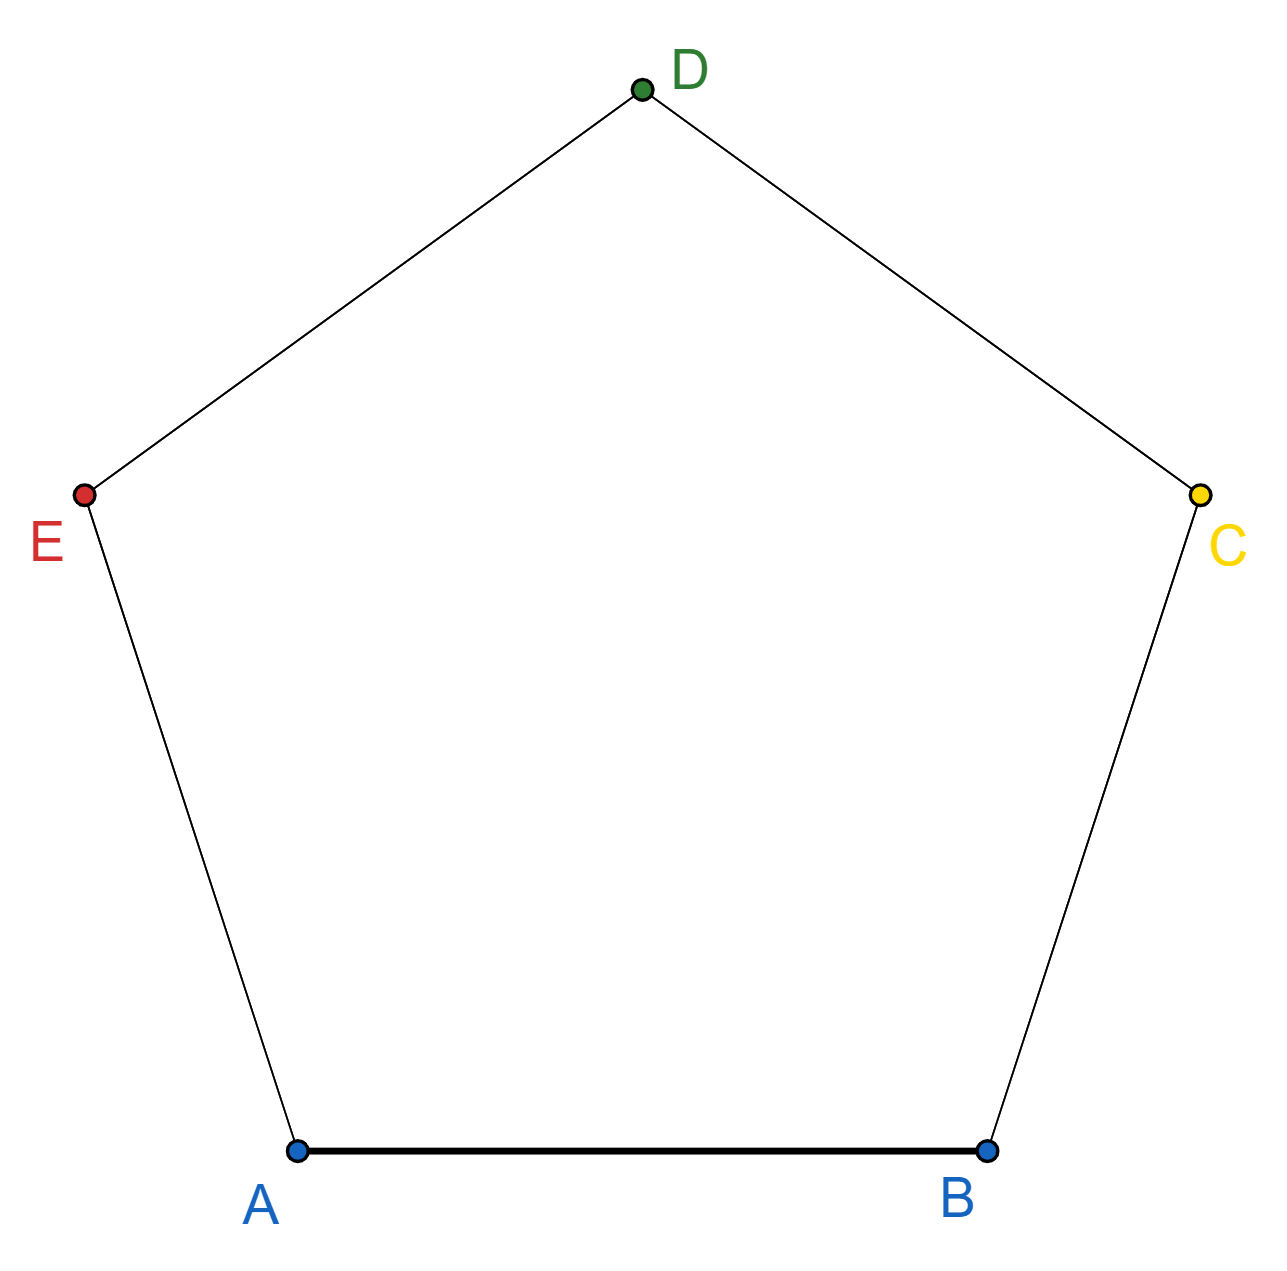
\includegraphics[scale=0.8]{geogebra-export.png}
                \caption{Diagram for $\mathcal{P}_\chi=\{\{0,4\},\{1\},\{2\},\{3\}\}$}
                \label{fig_diagn4}
            \end{center}
        \end{figure}
    \end{example}


    The diagram of a character defined above is useful because it will allow us to determine $S_{\chi,\aff}$ easily. The first step towards this goal is to associate elements of $\widetilde{W}_\chi$ to paths in the diagram.

    \begin{definition}
        Let $\mathfrak{D}_\chi$ be the diagram associated to $\chi$ and let $i,j\in\{0,1,\ldots,n\}$ be two \textit{distinct} vertices, and we assume that $i<j$. Let 
        $$\alpha_{i,j}=\alpha_{i+1}+\cdots+\alpha_{j-1}+\alpha_j\in\Phi^+$$
        be the positive root associated to the pair $(i,j)$. Let $T_{i,j,1}$, (resp. $T_{i,j,0}$) be the trail in $\mathfrak{D}_\chi$ from $i$ to $j$ avoiding (resp. passing through) the distinguished edge $e=\{0,n\}$. Then the associated reflection $w(T_{i,j,k})$ to the path $T_{i,j,k}$ is
        \begin{equation*}
            w(T_{i,j,k})=
            \begin{cases}
                w_{\alpha_{i,j}}(1) &\text{ if } k=1,\\
                w_{\alpha_{i,j}}(\varpi^{-1}) &\text{ if } k=0.
            \end{cases}
        \end{equation*}
    \end{definition}

    \begin{lemma}
        For any path $T_{i,j,k}$, we have that 
        $$l(w(T_{i,j,k}))=2l(T_{i,j,k})-1,$$
        where the length of a trail is the number of edges on the trail.
    \end{lemma}
    \begin{proof}
        Assume without loss of generality that $i<j$. 
        If $k=0$, then $l(T_{i,j,0})=j-i$, while Lemma \ref{lem_w1} shows that $l(w_{\alpha_{i,j}}(1))=2(j-i)+1$. If $k=1$, we may use Corollary \ref{cor_lengthsum} to obtain
        $$l(w_{\alpha_{i,j}}(\varpi^{-1}))=2n-l(w_{\alpha_{i,j}}(1))=2n-2l(T_{i,j,0})+1=2(n+1-l(T_{i,j,0}))-1=2l(T_{i,j,1})-1,$$
        and this concludes the lemma.
    \end{proof}

    \begin{proposition}\label{prop_Schi}
        Let $\chi$ be a depth-zero character of $T(\cO)$ and let $\mathfrak{D}_\chi$ be the associated diagram induced by the partition $\mathcal{P}_\chi=\{A_1,\ldots,A_r\}$ of its vertices. For each set $k\in\{1,\ldots,r\}$, write $A_k=\{a_{k,1}<\cdots<a_{k,m_k}\}$ and let $\{T_{k,i}\ |\ i=1,\ldots,m_k\}$ be all the paths joining each consecutive pair of vertices in $A_k$. Then
        \begin{equation*}
            S_{\chi,\aff}=\bigcup_{k=1}^r \{w(T_{k,1}),\ldots,w(T_{k,m_k})\}.
        \end{equation*}
    \end{proposition}

    \begin{proof}
        Firstly, we note that if $\mathcal{P}_\chi=\{A_1,\ldots,A_r\}$, which each $A_k$ of size $m_k$, then 
        $$\widetilde{W}_\chi\cong \widetilde{W}_{\chi^{(1)}}\times\cdots\times\widetilde{W}_{\chi^{(r)}},$$
        where $\chi^{(k)}=\chi_{a_{k,1}}\otimes\cdots\otimes\chi_{a_{k,m_k}}$ is the depth-zero character of $\GL_{m_k}$, and $\widetilde{W}_{\chi^{(k)}}$ is viewed as a subgroup of $\widetilde{W}_{\chi}$ in the obvious way. Each $\widetilde{W}_{\chi^{(k)}}$ is isomorphic to the extended Weyl group of $\GL_{m_k}$, and if we let $S_{\chi,\aff,k}$ be the set of simple reflections of $\widetilde{W}_{\chi^{(k)}}$ viewed as a subgroup of $\widetilde{W}_{\chi}$, then 
        $$S_{\chi,\aff}=\bigcup_{k=1}^r S_{\chi,\aff,k}.$$
        It therefore suffices to show that 
        $$S_{\chi,\aff,k}=\{w(T_{k,1}),\ldots,w(T_{k,m_k})\}.$$
        \textcolor{red}{still remains to prove this, which is definitely expected to be true!}
    \end{proof}
        
    \subsection{The induced homomorphism on Hecke algebras}

    Having established a way to easily determine $S_{\chi,\aff}$ from the character $\chi$, in this subsection we construct, for each depth-zero character $\chi$ and $s\in S_{\chi,\aff}$, a homomorphism of $p$-adic groups $\psi_s$ with certain nice properties that induce a homomorphism on Hecke algebras. This homomorphism $\psi_s$ will be our main tool to deduce the quadratic equation for $\varphi_s=q^{(1-l(s))/2}[IsI]_{\check{\chi}}$ from our results in the previous section.

    Before we can construct these homomorphisms, we first need to consider the element
    \begin{equation*}
        \rho_n:=
        \begin{pmatrix}
            &1&& \\
            &&\ddots& \\
            &&&1 \\
            -\varpi&&& 
        \end{pmatrix}
        \in\GL_{n+1}(F),
    \end{equation*}
    which is the generator of the alcove stabilizer $\Omega$. This element has a natural action on the set of depth-zero characters of $T(\cO)$ that is compatible with a certain action on the diagrams.

    \begin{lemma}
        The action of $\rho_n$ on the space of depth-zero characters of $T(\cO)$ is compatible with a clockwise rotation of $2\pi/n$ radians on the coloring of the diagrams.
        
        In other words, if $\chi$ is a depth-zero character of $T(\cO)$, then $\prescript{\rho_n}{}{\chi}(\cdot)=\chi(\rho_n^{-1}\cdot\rho_n)$ is another depth-zero character. Moreover,        
        $$\mathfrak{D}_{\prescript{\rho_n}{}{\chi}}=r_n(\mathfrak{D}_\chi)\quad\text{and}\quad S_{\prescript{\rho_n}{}{\chi},\aff}=\rho_n S_{\chi,\aff}\rho_n^{-1},$$
        where $r_n(\mathfrak{D})$ is obtained by rotating the coloring of $\mathfrak{D}$ clockwise $2\pi/(n+1)$ radians.
    \end{lemma}
    \begin{proof}
        We first note that 
        \begin{equation}\label{eqn:rhon}
            \rho_n^{-1}
            \begin{pmatrix}
                a_0&&&\\
                &a_1&&\\
                &&\ddots&\\
                &&&a_n
            \end{pmatrix}
            \rho_n=
            \begin{pmatrix}
                a_n&&&\\
                &a_0&&\\
                &&\ddots&\\
                &&&a_{n-1}
            \end{pmatrix}.
        \end{equation}
        Therefore, if $\chi=\chi_0\otimes\chi_1\otimes\cdots\otimes\chi_n$, then $\prescript{\rho_n}{}{\chi}=\chi_1\otimes\cdots\otimes\chi_n\otimes\chi_0$, and by construction, $\mathfrak{D}_{\prescript{\rho_n}{}{\chi}}=r_n(\mathfrak{D}_\chi)$.
    \end{proof}


    Now we are ready to construct a homomorphism $\psi_s$ of $p$-adic groups associated to $s\in S_{\chi,\aff}$, where $\chi$ is some depth-zero character of $T(\cO)\subseteq\GL_{n+1}(F)$. By Proposition \ref{prop_Schi}, the reflection $s$ corresponds to some trail $T_s$ connecting two distinct vertices $i$ and $j=i+l\pmod{n+1}$ of $\mathfrak{D}_\chi$ \textbf{counterclockwise} and with length $l=(1+l(s))/2\leq n$. Then define
    \begin{align}\label{eqn_psis}
        \psi_s:\GL_{l+1}(F)&\longrightarrow\GL_{n+1}(F)\\
        A&\longmapsto\rho_n^{n+1-i}
        \begin{pmatrix}
            A&\\
            & \Id_{n-l}
        \end{pmatrix}\rho_n^{i-n-1},
    \end{align}
    which is clearly a continuous homomorphism of $p$-adic groups. Note that $\psi_s$ is the composition of the two homomorphisms
    \begin{align*}
        \phi_{l,n}:\GL_{l+1}(F)&\longrightarrow\GL_{n+1}(F)&\text{and}\quad\phi_s:\GL_{n+1}(F)&\longrightarrow\GL_{n+1}(F)\\
        A&\longmapsto
        \begin{pmatrix}
            A&\\
            &\Id_{n-l}
        \end{pmatrix}
        &B&\longmapsto\rho_n^{n+1-i}
        B\rho_n^{i-n-1}.
    \end{align*}
    We remark that if $\chi=\chi_0\otimes\cdots\otimes\chi_n$ with $\chi_0=\chi_n$ and all the other $\chi_i$ distinct (as in the previous section) and $s=w_{\alpha_0}(1)\in S_{\chi,\aff}$, then $\psi_s$ is the identity map on $\GL_{n+1}(F)$.

    \begin{lemma}
        For any depth-zero character $\chi$ of $T(\cO)\subset\GL_{n+1}$ and any $s\in S_{\chi,\aff}$, the homomorphism $\psi_s:\GL_{l+1}(F)\longrightarrow\GL_{n+1}(F)$ satisfies the following properties:
        \begin{enumerate}
            \item $\psi_s^{-1}(T(\cO))=T(\cO)$ and $\psi_s^{-1}(N)=N$,
            \item $\psi_s^{-1}(I)=I$.
        \end{enumerate}
    \end{lemma}

    \begin{proof}
        Both properties are immediate for the homomorphism $\phi_{l,n}$. The map $\phi_s$ is an isomorphism, and it preserves the $\cO$-points of the torus $T$ and the normalizer of the tori $N$ since $\rho_n\in N(F)=N_G(T(\cO))$. It also preserves the Iwahori subgroup $I$ since $\rho_n$ is a fundamental alcove stabilizer. This concludes the proof.
    \end{proof}

    The previous lemma shows that $\psi_s$ induces a homomorphism of extended Weyl groups $\overline{\psi}_s:\widetilde{W}_{l+1}\rightarrow\widetilde{W}_{n+1}$. If $s$ corresponds to a trail $T_s$ on $\mathfrak{D}_\chi$ connecting the vertices $i$ and $j=i+l\pmod{n+1}$ in $\mathfrak{D}_\chi$, we consider the character $$\chi^{(s)}:=\chi_i\otimes\chi_{i+1}\otimes\cdots\otimes\chi_{j-1}\otimes\chi_j$$
    of $T(\cO)\subset\GL_{l+1}(F)$, where subscripts are taken mod $n+1$. The following two results provide two fundamental properties of the character $\chi^{(s)}$.

    \begin{lemma}\label{lem_hompsi_s}
        The homomorphism $\overline{\psi}_s$ satisfies 
        \begin{equation*}
            \overline{\psi}_s(\widetilde{W}_{\chi^{(s)}})\subseteq\widetilde{W}_\chi\quad\text{and}\quad\overline{\psi}_s(w_{\beta_0}(1))=s,
        \end{equation*}
        where $\beta_0$ is the highest root of $\GL_{l+1}$.
    \end{lemma}
    \begin{proof}
        We note that $\psi_s=\phi_s\circ\phi_{l,n}$ and that both $\phi_s$ and $\phi_{l,n}$ also induce maps of Weyl groups such that 
        $\overline{\psi}_s=\overline{\phi}_s\circ\overline{\phi}_{l,n}$. 
        By definition of $\phi_{l,n}$, we can see that $$\overline{\phi}_{l,n}(\widetilde{W}_{\chi^{(s)}})\subseteq\widetilde{W}_{\chi'},\quad\text{where}\quad\chi'=\chi^{(s)}\otimes\chi_{j+1}\otimes\cdots\otimes\chi_{i-1}=\prescript{\rho_n^i}{}{\chi}$$
        and that 
        $$\overline{\phi}_{l,n}(w_{\beta_0}(1))=w_{\alpha_1+\cdots+\alpha_l}(1),$$ 
        which corresponds to the trail in $\mathfrak{D}_\chi$ connecting $0$ and $l$ counterclockwise. On the other hand $\overline{\phi}_s(w)=\rho_n^{n+1-i}w\rho_n^{i-n-1}$ for any $w\in\widetilde{W}_{n+1}$, so $$\overline{\phi}_s(\widetilde{W}_{\chi'})=\widetilde{W}_{\prescript{\rho_n^{-i}}{}{\chi'}}=\widetilde{W}_\chi.$$

        Moreover, 
        $$\overline{\phi}_s(w_{\alpha_1+\cdots+\alpha_l}(1))=\rho_n^{n+1-i}w_{\alpha_1+\cdots+\alpha_l}(1)\rho_n^{i-n-1}$$
        corresponds to the trail $T_s$ in $\mathfrak{D}_\chi$ connecting $i$ and $j=i+l\pmod{n+1}$ counterclockwise. Thus,
        $$\overline{\psi}_s(w_{\beta_0}(1))=\overline{\phi}_s(\overline{\phi}_{l,n}(w_{\beta_0}(1)))=\overline{\psi}_s(w_{\alpha_1+\cdots+\alpha_l}(1))=s\quad\quad\text{and}\quad\quad\overline{\psi}_s(\widetilde{W}_{\chi^{(s)}})\subseteq\overline{\phi}_s(\widetilde{W}_{\chi'})=\widetilde{W}_\chi,$$
        as desired.
    \end{proof}

    %Given a depth-zero character $\chi=\chi_0\otimes\cdots\otimes\chi_n$ of $T(\cO)\subset\GL_{n+1}(F)$ and $s\in S_{\chi,\aff}$ connecting the vertices $i$ and $j=i+l\pmod{n+1}$ in $\mathfrak{D}_\chi$, define the character $$\chi^{(s)}=\chi_i\otimes\chi_{i+1}\otimes\cdots\otimes\chi_{j-1}\otimes\chi_j$$
    %of $T(\cO)\subset\GL_{l+1}(F)$, where subscripts are taken mod $n+1$. 

    \begin{lemma}\label{lem_compatible-rho}
        For any $k\in I\subset\GL_{l+1}(F)$, 
        $$\rho_\chi(\psi_s(k))=\rho_{\chi^{(s)}}(k).$$
    \end{lemma}
    \begin{proof}
        Fix some $k\in I\subset\GL_{l+1}(F)$ and let $\chi=\chi_0\otimes\cdots\otimes\chi_n$.
        By definition of $\phi_{l,n}$, we have that
        $$\rho_\chi(\phi_{l,n}(k))=\rho_{\chi'}(k),$$
        where $\chi'=\chi_0\otimes\cdots\otimes\chi_l$ is obtained from $\chi$ by taking the characters of the first $l+1$ entries. Moreover, since conjugating by $\rho_n$ permutes the diagonal entries according to \eqref{eqn:rhon}, it follows that for any $h\in I\subset\GL_{n+1}$, 
        $$\rho_\chi(\rho_n^{-1}h\rho_n)=\rho_{\prescript{\rho_n}{}{\chi}}(h),\quad\text{where}\quad\prescript{\rho_n}{}{\chi}=\chi_1\otimes\cdots\otimes\chi_n\otimes\chi_0.$$
        Therefore, by the construction of $\phi_s$, we have that 
        $$\rho_\chi(\phi_s(h))=\rho_{\prescript{\rho_n^i}{}{\chi}}(h),\quad\text{where}\quad\prescript{\rho_n^i}{}{\chi}=\chi_i\otimes\chi_{i+1}\otimes\cdots\otimes\chi_{i-1}.$$
        Putting everything together, we obtain
        $$\rho_\chi(\psi_s(k))=\rho_\chi(\phi_s(\phi_{l,n}(k)))=\rho_{\prescript{\rho_n^i}{}{\chi}}(\phi_{l,n}(k))=\rho_{\chi^{(s)}}(k),$$
        as desired.
    \end{proof}

    We are finally ready to prove the existence of a surjective algebra homomorphism between Hecke algebras.

    \begin{proposition}\label{prop_algebrahom}
        The homomorphism $\psi_s$ induces a surjective Hecke algebra homomorphism 
        \begin{equation*}
            \Psi_s:\cH(\GL_{n+1},I,\rho_\chi)\longrightarrow\cH(\GL_{l+1},I,\rho_{\chi^{(s)}}),
        \end{equation*}
        where
        $$\Psi_s(\varphi)(g)=\varphi(\psi_s(g)),\quad\quad \varphi\in\cH(\GL_{n+1},I,\rho_\chi),\ g\in\GL_{l+1}(F).$$
        Furthermore, for every $w\in\widetilde{W}_{\chi^{(s)}}$,
        $$\Psi_s([I\overline{\psi}_s(w)I])=[IwI].$$
    \end{proposition}
    \begin{proof}
        For any $\varphi\in\cH(\GL_{n+1},I,\rho_\chi)$, we have that $\supp(\Psi_s(\varphi))=\psi_s^{-1}(\supp(\varphi))$, a compact subset of $\GL_{l+1}(F)$ since $\psi_s$ is a continuous map. Moreover, if $k_1,k_2\in I\subset\GL_{l+1}(F)$ and $g\in\GL_{l+1}(F)$, then by Lemma \ref{lem_compatible-rho}
        $$\Psi_s(\varphi)(k_1gk_2)=\varphi(\psi_s(k_1gk_2))=\rho_\chi(\psi_s(k_1))\varphi(\psi_s(g))\rho_\chi(\psi_s(k_2))=\rho_{\chi^{(s)}}(k_1)\Psi_s(g)\rho_{\chi^{(s)}}(k_2),$$
        so $\Psi_s(\varphi)\in\cH(\GL_{l+1},I,\rho_{\chi^{(s)}})$. 

        \textcolor{red}{By Lemma \ref{lem_hompsi_s}, $\overline{\psi}_s(w)\in \widetilde{W}_{\chi}$ for any $w\in\widetilde{W}_{\chi^{(s)}}$ and since $\psi_s$ is an injective homomorphism,
        \begin{equation*}
            \Psi_s\left([I\overline{\psi}_s(w)I]\right)(g)=[I\overline{\psi}_s(w)I](\psi_s(g))=
            \begin{cases}
                [IwI](g)&\text{ if }g\in IwI,\\
                0 &\text{ otherwise}.
            \end{cases}
            =[IwI](g)
        \end{equation*}}
        
        This also implies that the map $\Psi_s$ is surjective since $\{[IwI]\ |\ w\in\widetilde{W}_{\chi^{(s)}}\}$ is a $C$-basis of $\cH(\GL_{l+1},I,\rho_{\chi^{(s)}})$.
        Finally, to show that $\Psi_s$ is an algebra homomorphism, we compute, for each $\varphi_1,\varphi_2\in\cH(\GL_{n+1},I,\rho_\chi)$ and $g\in\GL_{l+1}(F)$,
        \begin{align*}
            \Psi_s(\varphi_1*\varphi_2)(g)&=(\varphi_1*\varphi_2)(\psi_s(g))=\int_{\GL_{n+1}}\varphi_1(\psi_s(g)h)\varphi_2(h^{-1})dh
            =\int_{\GL_{l+1}}\varphi_1(\psi_s(g)\psi(h))\varphi_2(\psi_s(h)^{-1})dh\\
            &=\int_{\GL_{l+1}}\Psi_s(\varphi_1)(gh)*\Psi_s(\varphi_2)(h^{-1})dh=\Psi_s(\varphi_1)*\Psi_s(\varphi_2)(g),
        \end{align*}
        as desired.
    \end{proof}

    With the previous proposition, we now have all the ingredients to prove the quadratic relation for $\varphi_s=q^{(1-l(s))/2}[IsI]_{\check{\chi}}\in\cH(\GL_{n+1})$. 

    \begin{theorem}
        Let $\chi=\chi_0\otimes\cdots\otimes\chi_n$ be a depth-zero character of $T(\cO)\subset\GL_{n+1}$ and let $s\in S_{\chi,\aff}$. If $$\varphi_s=q^{\frac{1-l(s)}{2}}[IsI]_{\check{\chi}}\in\cH(\GL_{n+1},I,\rho_\chi),$$
        then
        $$\varphi_s^2=(q-1)\varphi_s+q\varphi_1.$$
    \end{theorem}
    \begin{proof}
        Consider the algebra homomorphism $\Psi_s:\cH(\GL_{n+1},I,\rho_\chi)\longrightarrow\cH(\GL_{l+1},I,\rho_{\chi^{(s)}})$, and by Proposition \ref{prop_algebrahom} we have that 
        \begin{align*}
            \Psi_s(\varphi_s)=q^{\frac{(1-l(s))}{2}}\Psi_s([IsI]_{\check{\chi}})&=q^{\frac{(1-l(s))}{2}}\Psi_s([I\overline{\psi}_s(w_{\beta_0}(1))I]_{\check{\chi}})\\
            &=q^{\frac{(1-l(w_{\beta_0}(1)))}{2}}[Iw_{\beta_0}(1)I]=\varphi_{w_{\beta_0}(1)}\in\cH(\GL_{l+1},I,\rho_{\chi^{(s)}}).
        \end{align*}
        By the results on the previous section, we know that $\varphi_{w_{\beta_0}(1)}$ satisfies the desired quadratic relation, and since $\Psi_s$ is an algebra homomorphism, it follows that 
        $$\varphi_s^2-(q-1)\varphi_s-q\varphi_1\in\ker\Psi_s\cap \Span_C\{\varphi_1,\varphi_s\}.$$
        However, $\Psi_s(\varphi_s)=\varphi_{w_{\beta_0}(1)}$ and $\Psi_s(\varphi_1)=\varphi_1$, which are non-zero and linearly independent in $\cH(\GL_{l+1},I,\rho_{\chi^{(s)}})$. Thus, $\ker\Psi_s\cap \Span_C\{\varphi_1,\varphi_s\}=\{0\}$, yielding  
        $$\varphi_s^2=(q-1)\varphi_s+q\varphi_1$$
        and this concludes the proof.
    \end{proof}


    
    

\end{document}